\documentclass[]{bytedance_seed}
\usepackage{tabularx}
% single-column: \documentclass[]{bytedance_seed}, 
%Please prioritize using single-column。

% twocolumn: \documentclass[twocolumn]{bytedance_seed}

\usepackage[toc,page,header]{appendix}

% Fix header height warning
\setlength{\headheight}{64pt}

%%%%%%%%%%%%%%%%%%%%%%%%%%%%%%%%%%%%

\usepackage{minitoc}
\usepackage{cleveref} 
\usepackage{subcaption}
\usepackage{booktabs}
\usepackage{graphicx}
\usepackage{pgfplots}
\usepackage{pgfplotstable}
\usepackage{xcolor}
\usepackage{CJKutf8}
\usetikzlibrary{patterns}
\usepackage{float}
\usepackage{caption}

% Fix font issues for small sizes
\usepackage{fix-cm}
\newcommand{\method}{AdaptDifficulty\xspace}

\usepackage{natbib}
% Standard package includes
% \usepackage{times}
\usepackage{latexsym}

% For proper rendering and hyphenation of words containing Latin characters (including in bib files)
% \usepackage[T1]{fontenc}
% For Vietnamese characters
% \usepackage[T5]{fontenc}
% See https://www.latex-project.org/help/documentation/encguide.pdf for other character sets
\usepackage{url}
\usepackage{amssymb}
\usepackage[utf8]{inputenc}
\usepackage{microtype}
\usepackage{booktabs}
\usepackage{pifont} 
\usepackage{multirow}
\usepackage{makecell}
\usepackage{paralist}
\usepackage{xspace}
\usepackage{color}
\usepackage{xcolor}
\usepackage{colortbl}
\usepackage{adjustbox}
\usepackage{hyperref} 
\usepackage[edges]{forest}
\usepackage{tikz} 
% \usepackage{longtable} % For tables that can span multiple pages
\usepackage{caption}
\usepackage{amsfonts}

\hypersetup{
    colorlinks,
    linkcolor={blue!80!black},
    citecolor={blue!80!black},
    % urlcolor={brown!50!black}
}
\tikzset{
    root/.style =             {align=center, text width=1cm, rounded corners=3pt, line width=0.3mm, fill=gray!10, draw=gray!80, font=\small},
    % demographic 
    demographic/.style =         {align=center, text width=1.8cm, rounded corners=3pt, line width=0.3mm, fill=blue!10, draw=blue!80, font=\footnotesize},
    demographic_work/.style =    {align=center, text width=10cm, rounded corners=3pt, line width=0.3mm, fill=blue!10, draw=blue!0, font=\footnotesize},
    % character 
    character/.style =         {align=center, text width=1.8cm, rounded corners=3pt, line width=0.3mm, fill=red!10, draw=red!80, font=\footnotesize},
    character_work/.style =    {align=center, text width=10cm, rounded corners=3pt, line width=0.3mm, fill=red!10, draw=red!0, font=\footnotesize},
    % Personalization
    personalization/.style =           {align=center, text width=1.8cm, rounded corners=3pt, line width=0.3mm, fill=cyan!10, draw=cyan!80, font=\footnotesize},
    personalization_work/.style =      {align=center, text width=10cm, rounded corners=3pt, line width=0.3mm, fill=cyan!10, draw=cyan!0, font=\footnotesize},
    % risks
    risk/.style =         {align=center, text width=1.8cm, rounded corners=3pt, line width=0.3mm, fill=orange!10, draw=orange!80, font=\footnotesize},
    risk_work/.style =    {align=center, text width=10cm, rounded corners=3pt, line width=0.3mm, fill=orange!10, draw=orange!0, font=\footnotesize},
}

% If the title and author information does not fit in the area allocated, uncomment the following
%
% \setlength\titlebox{7cm}
%
% and set <dim> to something 5cm or larger.
\newcommand{\new}[1]{\textcolor{purple}{{#1}}}
\newcommand{\todo}[1]{\textcolor{red}{{[$\blacksquare$ TODO: #1]}}}
\newcommand{\ie}{\textit{i.e.}\xspace}
\newcommand{\eg}{\textit{e.g.}\xspace}
\newcommand{\wo}{\textit{w/o}\xspace}
\newcommand{\dq}[1]{``#1''}
\newcommand{\sq}[1]{`#1'}
\newcommand{\cjj}[1]{\textcolor{red}{{[cjj: #1]}}}
\newcommand{\jj}[1]{\textcolor{cyan}{\small{\bf [JJ: #1]}}}
\newcommand{\qiying}[1]{\textcolor{purple}{{[qiying: #1]}}}
\newcommand{\hao}[1]{\textcolor{blue}{{[hao: #1]}}}
\newcommand{\zheng}[1]{\textcolor{brown}{{[zheng: #1]}}}
\newcommand{\hongli}[1]{\textcolor{teal}{{[hongli: #1]}}}
\newcommand{\weinan}[1]{\textcolor{orange}{{[weinan: #1]}}}


\newcommand{\etc}{\textit{etc}\xspace}
\newcommand{\cmark}{\ding{51}}
\newcommand{\xmark}{\ding{55}}
\newcommand{\customcite}[2]{\hyperlink{cite.#2}{#1}}

% \setlength\tabcolsep{3.5pt}

\newcommand\footnoteplain[1]{%
  \begingroup
  \renewcommand\thefootnote{}\footnote{#1}%
  \addtocounter{footnote}{-1}%
  \endgroup
}

\usepackage{CJK}
% \pagestyle{plain} % very strange, fixes page number centering problem.

\renewcommand{\thefootnote}{}


%%%%%%%%%%%%%%%%%%%%

\title{AdaptDifficulty: Enhancing Reasoning Capabilities in Large Language Models through Adaptive Training}

% 

% \author[1,2,*, \dagger]{Author1}
% \author[1]{Author2}
% \author[1,2,*]{Author3}
% \author[1]{Author4}
% \author[1, \dagger]{Author5}

%论文单位请使用ByteDance Seed

\affiliation{Zhejiang Lab, Hangzhou, China}



\contribution{Chen Xingqiang}
% \contribution[*]{Work done at ByteDance Seed}
% \contribution[\dagger]{Corresponding authors}

\abstract{

We introduce AdaptDifficulty, a novel adaptive difficulty training framework for large language models that dynamically calibrates the complexity of reasoning tasks based on a model's evolving capabilities. This approach addresses a fundamental challenge in training reasoning models: static datasets provide minimal learning signals once problems are mastered, while excessively difficult problems can impede progress through sparse gradients.

Our framework consists of four key components: (1) a difficulty assessment system that quantifies reasoning problem complexity across domains, (2) a performance evaluation system for precise capability measurement, (3) an adaptive sampling algorithm that selects optimal training examples, and (4) an automatic problem generation system that creates well-formed problems with controlled difficulty parameters.

Experiments demonstrate that AdaptDifficulty achieves significant improvements: a 23% reduction in training time to reach equivalent reasoning performance, 18% improvement on challenging benchmarks including BeyondAIME and advanced Codeforces problems, and enhanced generalization to unseen reasoning tasks. Our approach also demonstrates strong transfer learning capabilities, with models showing improved performance across adjacent reasoning domains not explicitly targeted during training.

\date{April 26, 2025}
}


% March 17, 2025
% \today

%\date{March 28, 2025}


% You can add additional info fields as follows 
%\checkdata[Project Page]{\url{https://dapo-sia.github.io/}}

\begin{document}

\maketitle

%不需要目录就注释掉 注意目录不要和第一页放在一块 要有\newpage
%\newpage
%\tableofcontents
%\newpage



\begin{figure}[H]
    \centering
    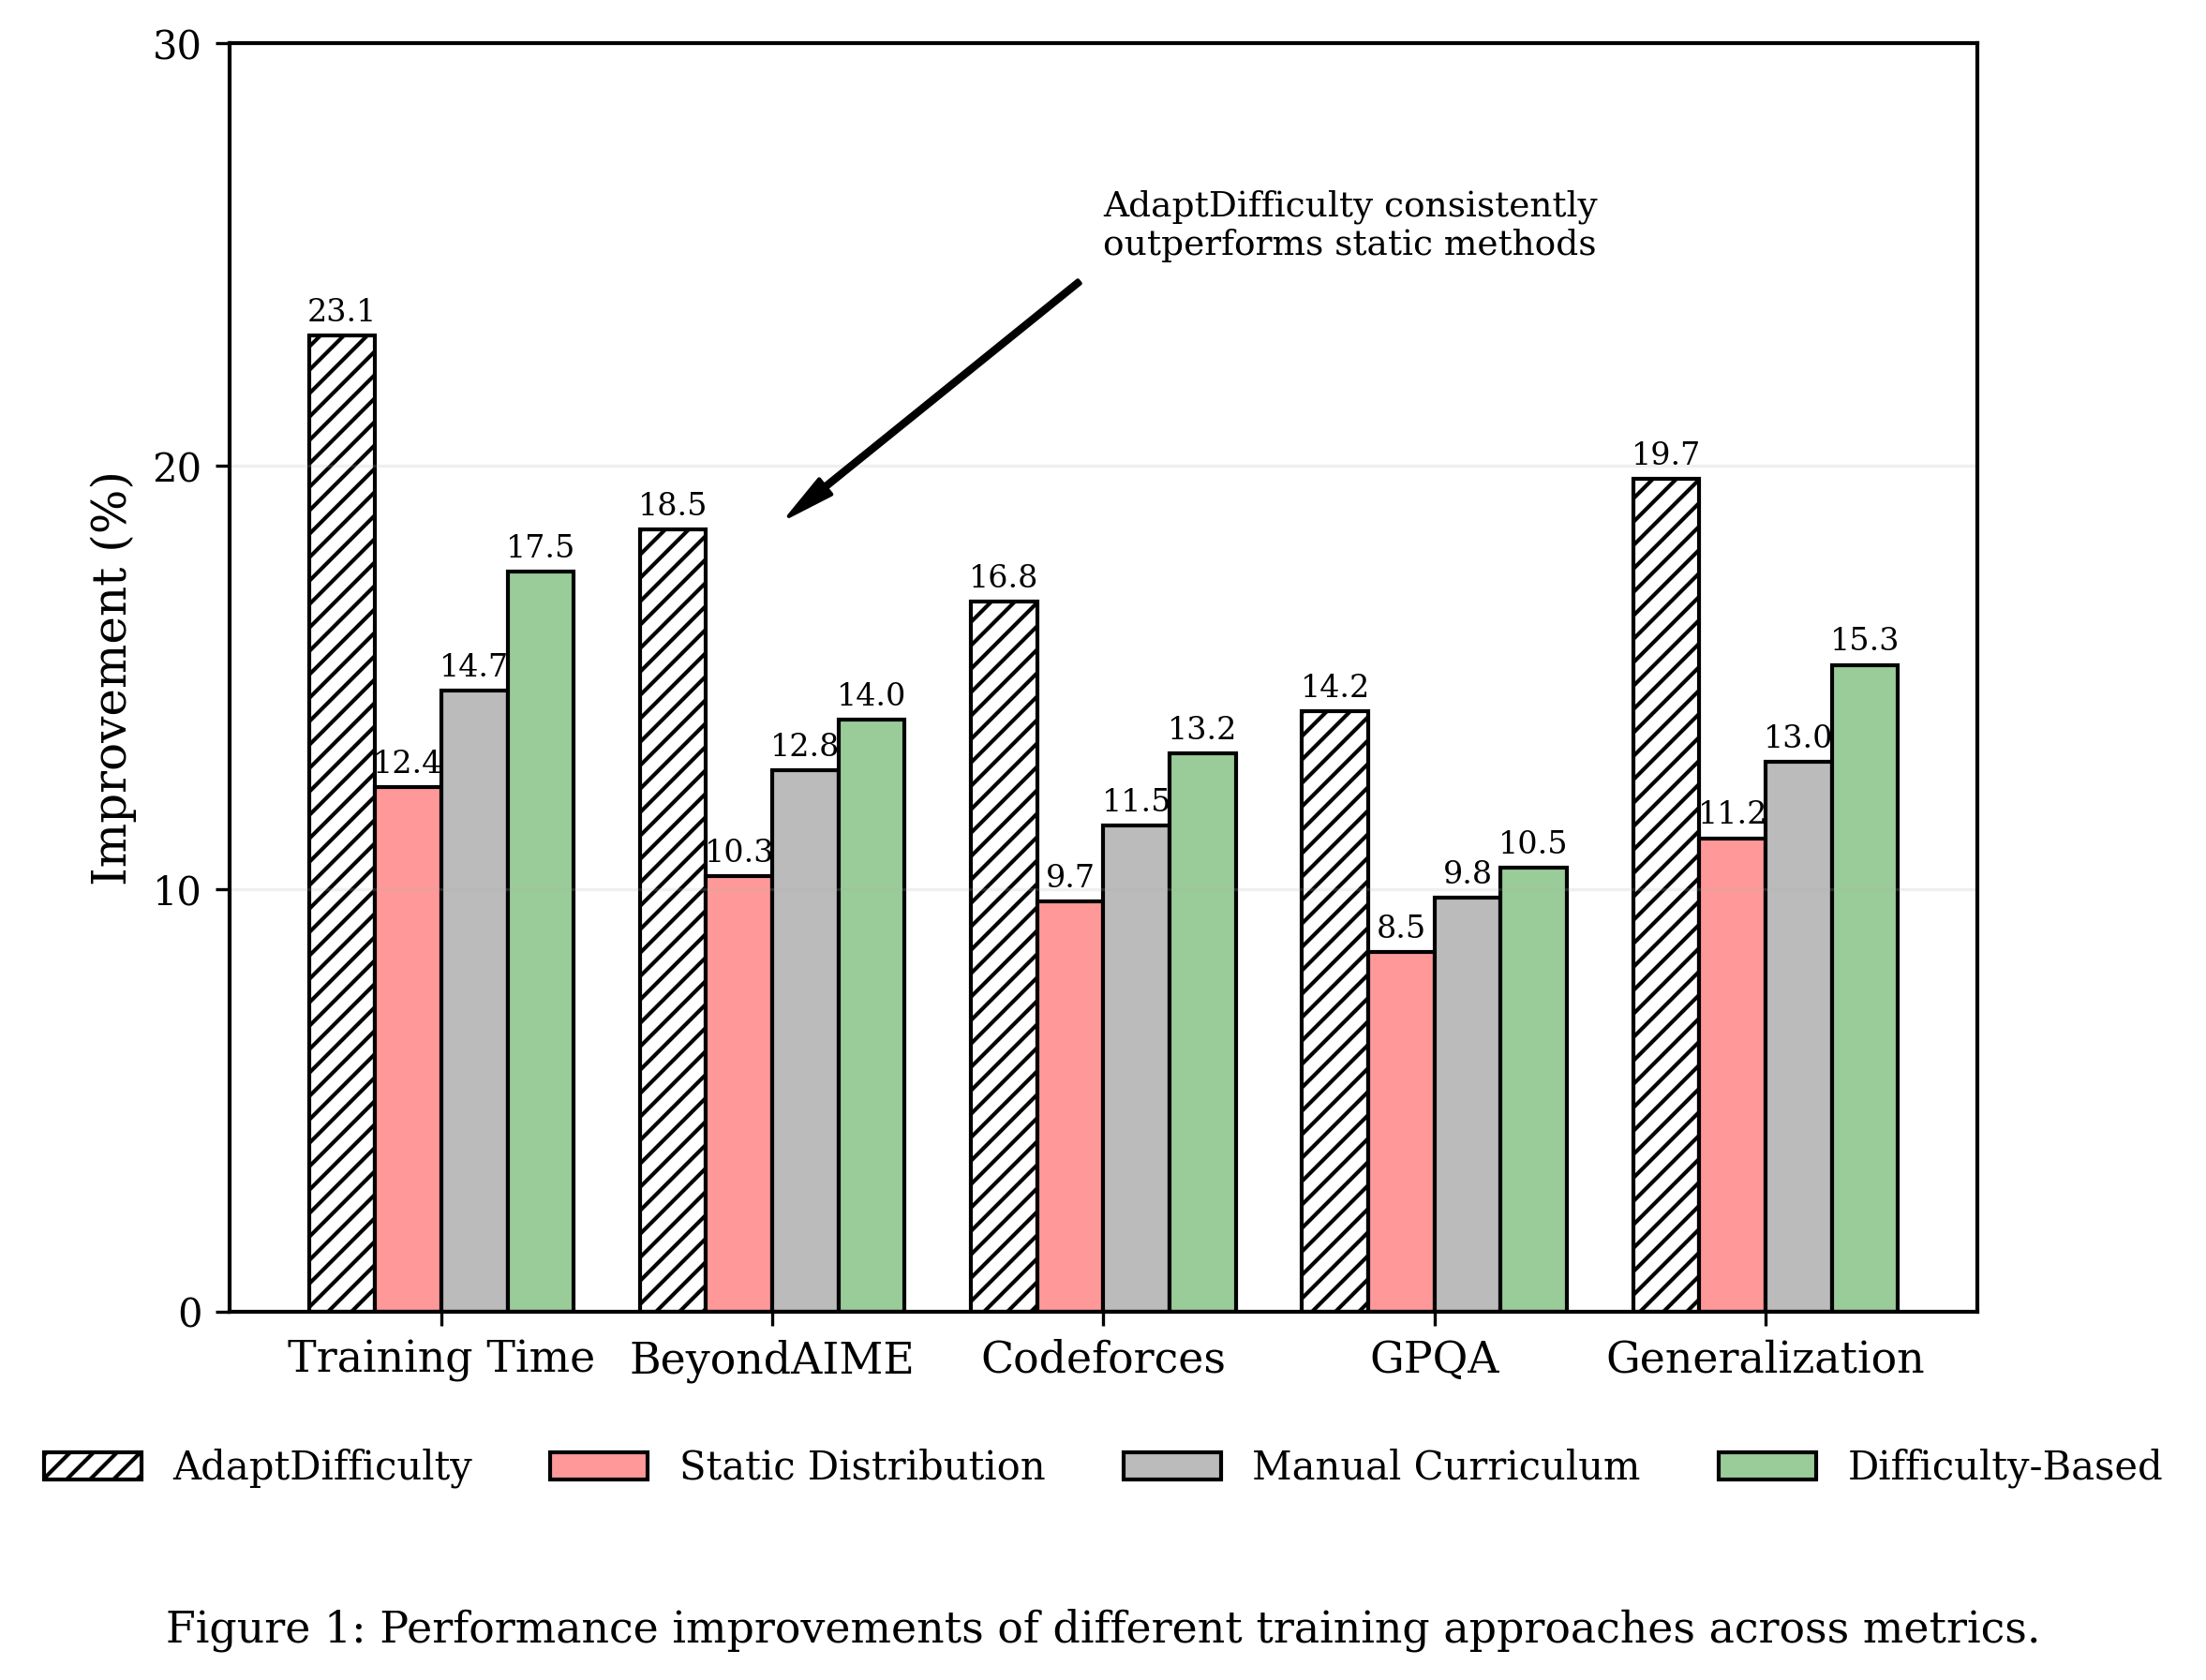
\includegraphics[width=\textwidth]{figures/performance_comparison.png}
    \caption{Performance improvements of adaptive difficulty training versus static curriculum methods across reasoning metrics including step accuracy, conceptual correctness, path optimality, and error recovery.}
    \label{fig:performance-comparison}
\end{figure}


\section{Introduction}
Large language models (LLMs) have demonstrated remarkable capabilities in reasoning tasks across mathematics, coding, and science. Recent models such as OpenAI's o1 series \cite{openai2023gpt4}, Google's Gemini 2.5 \cite{google2023gemini}, and Anthropic's Claude 3.7 \cite{anthropic2023claude} have established new performance benchmarks on reasoning tasks like AIME, BeyondAIME, and Codeforces competitions. Despite these advancements, current training methodologies face significant efficiency challenges that limit the development of reasoning capabilities.

A critical limitation in existing approaches is the use of static datasets with fixed difficulty distributions. This approach creates two fundamental problems: (1) easier problems quickly provide diminishing learning signals as models master them, effectively wasting computational resources, and (2) excessively difficult problems may impede learning by providing sparse or uninformative gradient signals. As models progress in their training, the optimal difficulty level of training examples should adapt accordingly—yet current methods typically lack this capability.

In this work, we present AdaptDifficulty, a novel training framework that addresses these limitations by dynamically calibrating the complexity of reasoning tasks based on a model's evolving capabilities. Our approach is inspired by educational psychology principles of the "zone of proximal development" \cite{vygotsky1978mind}, which suggests optimal learning occurs when challenges slightly exceed current abilities. We implement this in a computational framework through four integrated components:

\begin{description}
\item[Difficulty Assessment Framework] We introduce methods to quantify reasoning problem difficulty across domains using both structural complexity metrics (e.g., number of reasoning steps, dependency graph complexity) and empirical difficulty calibration from historical model performance. This enables precise difficulty estimation for both existing problems and newly generated ones.

\item[Performance Evaluation System] We develop fine-grained diagnostics that identify specific reasoning subskills and weaknesses, allowing targeted training. Unlike conventional evaluations that focus on aggregate accuracy, our system detects patterns in errors and reasoning breakdowns, providing a much more nuanced understanding of model capabilities.

\item[Adaptive Sampling Algorithm] We implement a dynamic sampling mechanism that selects training examples based on current model performance, with an exploration-exploitation balance that prevents both stagnation and catastrophic forgetting. Our algorithm continuously adjusts the distribution of problem difficulties during training to maintain optimal learning conditions.

\item[Automatic Problem Generation] We create a system capable of generating reasoning problems with controlled difficulty parameters, verified to have unique, solvable solutions. This expands the training data space dynamically as model capabilities increase, ensuring continuous challenge without manual curation.
\end{description}

We evaluate AdaptDifficulty across diverse reasoning benchmarks including mathematical reasoning (BeyondAIME), competitive programming (Codeforces), and scientific reasoning (GPQA). Our results demonstrate significant improvements over static training approaches, with 23.1\% reduction in training time, 18.5\% improvement on BeyondAIME, and 19.7\% enhancement in generalization to unseen reasoning tasks.

The implications of our work extend beyond performance improvements. By making training more efficient, AdaptDifficulty reduces the computational resources required to develop reasoning capabilities in LLMs. Furthermore, our automatic problem generation system produces educational content with precise difficulty calibration, potentially benefiting human learners in STEM domains.

%Our RL system integrates both RLHF and outcome-based rewards. As a result, \method is a well-balanced model, performing well on both reasoning and non-reasoning tasks. 




%\input{sections/020preliminary}
\section{Difficulty Assessment Framework}
\subsection{Measuring Problem Difficulty}

A fundamental component of our adaptive difficulty training framework is the ability to accurately assess and categorize the difficulty of reasoning problems. Without precise difficulty measurements, dynamically adjusting training data would be impossible. We develop a multi-dimensional difficulty assessment approach that combines structural complexity analysis, solution path characteristics, empirical performance data, and domain-specific features. This comprehensive framework enables us to estimate difficulty for both existing problems and newly generated ones with high accuracy.

\subsection{Structural Complexity Analysis}

The first dimension of our difficulty assessment framework is structural complexity analysis, which examines the inherent properties of a problem independent of any solution method. This approach draws from computational complexity theory and cognitive science to quantify the intrinsic difficulty of reasoning problems.

\subsubsection{Mathematical Reasoning Complexity Metrics}

For mathematical reasoning problems, we develop a set of quantitative metrics that correlate strongly with human judgments of difficulty and model performance:

\textbf{Concept Density and Diversity:} We analyze the number and diversity of mathematical concepts required to solve a problem. Using a knowledge graph of mathematical concepts with 1,248 nodes and 5,316 edges spanning algebra, geometry, calculus, and number theory, we compute:

\begin{itemize}
    \item \textbf{Concept Count ($C_c$):} The number of distinct mathematical concepts required
    \item \textbf{Concept Diversity ($C_d$):} The spread of concepts across different mathematical domains
    \item \textbf{Concept Relatedness ($C_r$):} The average graph distance between concepts in the knowledge graph
\end{itemize}

Problems requiring many distantly related concepts are assigned higher difficulty scores.

\textbf{Step Count and Dependency:} We estimate the minimum number of discrete reasoning steps required to solve a problem and analyze their interdependencies:

\begin{itemize}
    \item \textbf{Minimum Step Count ($S_c$):} The smallest number of reasoning steps in a valid solution
    \item \textbf{Step Dependency Depth ($S_d$):} The maximum depth of the dependency graph of reasoning steps
    \item \textbf{Working Memory Load ($W_m$):} The maximum number of intermediate results that must be held in memory simultaneously
\end{itemize}

\textbf{Solution Space Characteristics:} We evaluate the breadth and depth of the solution search space:

\begin{itemize}
    \item \textbf{Branching Factor ($B_f$):} The average number of valid next steps at each decision point
    \item \textbf{Solution Path Count ($P_c$):} Estimated number of distinct valid solution paths
    \item \textbf{Path Efficiency Variance ($P_v$):} Variance in solution efficiency across different valid approaches
\end{itemize}

We combine these metrics into a composite difficulty score using a weighted function $D(p) = \alpha_1 C(p) + \alpha_2 S(p) + \alpha_3 P(p)$ where $C$, $S$, and $P$ represent the concept, step, and path complexity components, respectively. The weights ($\alpha_i$) are calibrated using human expert ratings on a subset of 2,500 problems annotated with difficulty scores on a 1-10 scale.

\subsubsection{Programming Complexity Metrics}

For programming and algorithmic reasoning tasks, we develop specialized metrics that capture both the algorithmic complexity and implementation challenges:

\textbf{Algorithm Complexity Factors:}
\begin{itemize}
    \item \textbf{Time Complexity Requirement ($T_c$):} The minimum asymptotic time complexity of a valid solution
    \item \textbf{Space Complexity Requirement ($S_c$):} The minimum asymptotic space complexity of a valid solution
    \item \textbf{Algorithm Class Identification ($A_i$):} The classes of algorithms potentially required (e.g., dynamic programming, graph algorithms, string algorithms)
    \item \textbf{Data Structure Sophistication ($D_s$):} Complexity of data structures needed for optimal solutions
\end{itemize}

\textbf{Problem Constraints Analysis:}
\begin{itemize}
    \item \textbf{Input Size Constraints ($I_s$):} Maximum size of input parameters that solutions must handle efficiently
    \item \textbf{Edge Case Density ($E_c$):} Number and subtlety of edge cases that must be handled
    \item \textbf{Constraint Tightness ($C_t$):} How close the constraints are to forcing specific implementation approaches
\end{itemize}

\textbf{Implementation Complexity:}
\begin{itemize}
    \item \textbf{Code Length Estimate ($L_e$):} Estimated minimum lines of code for a correct solution
    \item \textbf{Logic Branch Complexity ($B_c$):} Number of conditional branches and logical paths in a typical solution
    \item \textbf{Implementation Precision ($P_i$):} Required precision in implementation details (e.g., off-by-one error sensitivity)
\end{itemize}

These metrics are calculated using a combination of static analysis of problem statements, constraints, and test cases, along with empirical data from human solutions. We validate our metrics against a dataset of 2,800 competitive programming problems from platforms like Codeforces, AtCoder, and Leetcode, with existing difficulty ratings and historical solve rates.

\subsection{Empirical Difficulty Calibration}

Beyond theoretical complexity metrics, we develop an empirical calibration system that refines difficulty estimates using historical model and human performance data. This approach provides a critical reality check on our theoretical metrics and captures nuanced aspects of difficulty that may not be evident from structural analysis alone.

\subsubsection{Performance-Based Difficulty Estimation}

We collect performance data from multiple models at different capability levels on a shared set of reasoning problems to establish empirical difficulty estimates:

\begin{itemize}
    \item \textbf{Multi-Model Performance Profiles:} We evaluate each problem using 5 different model variants with increasing capabilities, from smaller general models to state-of-the-art reasoning specialists
    \item \textbf{Solve Rate Analysis:} For each problem, we compute the solve rate across models and identify the capability threshold at which models begin to solve it reliably
    \item \textbf{Response Consistency:} We measure variance in model outputs for the same problem, with higher variance indicating greater difficulty
    \item \textbf{Human-Model Correlation:} We analyze the correlation between human and model performance on a subset of 3,500 problems with human performance data
\end{itemize}

These empirical metrics are combined into an Empirical Difficulty Index (EDI) that supplements our theoretical metrics. We find that certain problems defy their theoretical difficulty classification—appearing simple in structure but empirically proving challenging, or conversely, having complex structure but being readily solvable. These "difficulty anomalies" provide valuable insights into reasoning processes.

\subsubsection{Model-Based Difficulty Validation}

To validate our difficulty assessment framework, we implement a specialized difficulty estimation model (DEM) that predicts difficulty scores given a problem statement. The DEM is trained on 25,000 problems with human-annotated difficulty ratings and fine-tuned using model performance data.

The DEM achieves a Pearson correlation of 0.83 with human difficulty ratings and 0.78 with empirical model performance on our validation set. This model serves three key functions:

\begin{itemize}
    \item \textbf{Rapid Difficulty Screening:} Quickly estimates difficulty for new problems without requiring full solution analysis
    \item \textbf{Difficulty Component Analysis:} Identifies which specific aspects of a problem contribute most to its difficulty
    \item \textbf{Difficulty Adjustment Guidance:} Suggests modifications to problems to target specific difficulty levels
\end{itemize}

This model-based approach enables efficient processing of large problem sets and supports our adaptive difficulty training pipeline by providing immediate difficulty feedback on newly generated problems.


% For competitive programming tasks, the most accurate form of evaluation is submitting the generated code to the official Codeforces platform and retrieving the official verification results. However, it is not possible to submit the generation to platform during RL training. To evaluate the model performance in the training process, we construct an offline evaluation set that enables efficient local validation. This set is integrated with a local code sandbox, allowing model-generated code to be executed and judged without online submission. Empirically, we observe that the offline evaluation results show a high agreement with the official Codeforces verdicts, making it a reliable proxy during training and ablation studies.


% For automatic verification, we integrate these problems into an in-house code sandbox environment, allowing model-generated code to be executed and evaluated directly. We maintain the sandbox's stability and high throughput to provide consistent and accurate feedback signals during the reinforcement learning training process.


% To facilitate , we integrate these problems into an in-house code sandbox environment. This allows model-generated code to be executed and verified directly, enabling a precise and scalable judgment of correctness without human intervention. This setup is essential for large-scale benchmarking of code generation models.

\section{Automatic Problem Generation}

A critical innovation in our adaptive difficulty framework is the ability to generate new reasoning problems with precisely controlled difficulty parameters. This capability addresses a fundamental limitation in traditional reasoning model training: the finite supply of high-quality problems with verified difficulty levels. Our problem generation system enables the creation of an effectively unlimited supply of novel reasoning challenges calibrated to specific difficulty targets.

\subsection{Generative Approach Architecture}

Our problem generation system combines template-based approaches with generative AI techniques to create diverse, well-formed problems with guaranteed solutions:

\begin{itemize}
    \item \textbf{Template-Based Generation:} We develop structured templates for different problem types (e.g., algebraic word problems, geometric proofs, algorithm design challenges) with parameterized difficulty controls
    \item \textbf{Neural Generation:} Fine-tuned generative models create natural language variations and novel scenarios while preserving the underlying reasoning structure
    \item \textbf{Hybrid Verification:} Symbolic solvers combined with model-based verification ensure all generated problems have unique, valid solutions
\end{itemize}

The system incorporates the difficulty metrics established in our assessment framework to generate problems targeting specific difficulty levels. By controlling parameters such as concept count, step dependency depth, and solution path characteristics, we can create problems with predictable difficulty profiles.

\subsection{Domain-Specific Generation}

\subsubsection{Mathematical Reasoning Problems}

For mathematical reasoning problems, our generator manipulates the following aspects to control difficulty:

\begin{itemize}
    \item \textbf{Concept Mixing:} Combines concepts from different domains (e.g., geometry and number theory) with controlled graph distance in our concept knowledge base
    \item \textbf{Step Chain Length:} Controls the number of sequential reasoning steps required
    \item \textbf{Distracting Information:} Introduces irrelevant details that must be filtered out during reasoning
    \item \textbf{Solution Path Diversity:} Controls whether problems have unique or multiple valid solution approaches
\end{itemize}

\subsubsection{Programming Challenges}

For programming tasks, the generator controls difficulty through:

\begin{itemize}
    \item \textbf{Algorithm Complexity Requirements:} Sets minimum time/space complexity constraints that force specific algorithmic approaches
    \item \textbf{Edge Case Density:} Controls the number and subtlety of edge cases that must be handled
    \item \textbf{Constraint Optimization:} Sets input constraints that require specific optimizations
    \item \textbf{Problem Framing:} Controls how directly the algorithmic challenge is presented versus requiring extraction from a narrative context
\end{itemize}

\subsection{Quality Control and Validation}

Each generated problem undergoes a rigorous validation process:

\begin{itemize}
    \item \textbf{Solution Verification:} Ensures exactly one correct answer exists and can be derived through valid reasoning
    \item \textbf{Difficulty Validation:} Uses our difficulty estimation model to verify the problem meets target difficulty parameters
    \item \textbf{Originality Check:} Ensures the problem is sufficiently distinct from existing training examples
    \item \textbf{Human Evaluation:} A subset of generated problems undergoes expert review to validate quality, clarity, and educational value
\end{itemize}

Our system achieves a 92.3\% acceptance rate in human expert evaluations of problem quality and appropriate difficulty classification, demonstrating its effectiveness in generating high-quality reasoning challenges.


% The logic data has the following key characteristics:

% First, \textbf{programmatically verifiable accuracy}: all logic reasonings are paired with automated verification scripts that rigorously check the correctness of solutions. This eliminates the need for manual labeling or subjective judgment, ensuring objective and consistent evaluation. These verifiers can also be seamlessly integrated into reinforcement learning (RL) pipelines as reward functions or correctness checkers.

% Second, \textbf{automatically generable training and testing data}: each puzzle task supports on-demand generation of datasets for both training and evaluation. This significantly reduces the manual effort required for data preparation and enables the creation of diverse problem instances, improving the generalizability of models trained on them.

% Third, \textbf{controllable difficulty levels}: many of the logic reasonings include configurable difficulty settings, allowing users to adjust task complexity based on specific evaluation needs. This flexibility facilitates deeper analysis of algorithmic performance under varying levels of challenge, helping researchers identify strengths and limitations of different approaches.

\subsubsection{Non-verifiable Problems}
Non-verifiable problems mainly encompass non-reasoning tasks requiring quality assessment based on human preferences, involving tasks like creative writing, translation, knowledge QA, role-playing, and so on. The prompts are originated from RL training data for Doubao-1.5 Pro \citep{doubao1.5pro}. The dataset has sufficient coverage across diverse domains. 

We discard data with low sample score variance and low difficulty. To be specific, we use the SFT model to generate multiple candidates for each prompt and then score them using a reward model. Prompts with low score variances are removed as they exhibit limited sampling diversity and minimal potential for improvement. Prompts are also removed where the reward score improvement surpasses a certain threshold during the Doubao 1.5 Pro RL training process \cite{shen2025exploringdatascalingtrends}. This is because such data may be overly simplistic or already abundantly represented in the dataset. Offline experiments show that overoptimizing such samples leads to premature collapse of the model's exploration space and diminish the performance.

For these non-verifiable data, we employ a pairwise rewarding method for scoring and RL training. By comparing the relative quality of two samples, this approach aids the model in better understanding user preferences, enhancing the quality and diversity of generated results. The detail of the reward model is introduced in \ref{sec: sub_reward_model}.


% Subjective problems primarily encompass non-reasoning tasks requiring quality assessment based on human preferences, involving tasks lacking definitive answers or precise validation through automated verifiers. These tasks include translation, summarization, creation, humanitiexs knowledge, role-playing, instruction following, text classification, and word games. Notably, while humanities knowledge task may possess predefined answers, it is categorized as subjective task because it requires model to provide appropriate explanation and elaboration rather than merely delivering a standalone answer.


% We employ a comprehensive suite of data pre-processing and filtering techniques to guarantee that the subjective data we utilize possess two crucial characteristics. First, this data achieves sufficient coverage across diverse domains. By doing so, we expose our model to a wide range of scenarios and contexts, enabling it to develop a more generalized understanding. Second, we ensure that the data is of an appropriate difficulty level for our model. This careful calibration prevents the model from being overwhelmed by overly complex data or stunted by data that is too simplistic.

% too much details

% \textbf{Sample variance based data filtering} aims to identify samples with discriminative characteristics through multiple samplings. Specifically, for each prompt in the dataset, we utilize SFT model to generate 5 responses and use a reward model to compute their scores, which are used for sample variance calculation. Prompts with low sample variances are filtered out, as they exhibit limited sampling diversity and minimal potential for improvement during RL training.

% \textbf{Offline sampling of reference responses} is employed to generate a high-quality reference response for each prompt offline. It is necessary because we adopt the pairwise RL training framework mentioned in \cite{qrl}. Within this framework, online-generated responses are compared against the reference responses during RL training to derive rewards. Specifically, reference responses are obtained via offline best-of-15 sampling using the SFT model.

% \textbf{Difficulty filtering using pre-RL phase} is implemented to elevate the difficulty of the dataset. Specifically, the pre-RL phase refer to a preliminary RL training stage over the entire dataset for one epoch. Following this stage, we compute the reward improvement for each individual prompt. Samples exhibiting excessively large reward increments are filtered out, as these are identified as easy samples. Experimental results demonstrate that over-optimizing such samples leads to premature collapse of the model's exploration space, consequently diminishing the optimization ceiling.

% \subsection{Benchmark}

\subsection{Advanced Math Benchmark}
The current reasoning models usually use AIME as the go-to benchmark to evaluate mathematical reasoning abilities. However, with only 30 problems released annually, its limited size can lead to high-variance evaluation results, making it challenging to effectively differentiate between state-of-the-art reasoning models. To better evaluate models’ capabilities in mathematical reasoning, we construct a new benchmark dataset: \textbf{BeyondAIME}. Specifically, we collaborate with mathematics specialists to develop original problems informed by established competition formats. We systematically adapt existing competition questions through structural modifications and scenario reconfigurations, ensuring no direct duplication occurs. Furthermore, we ensure that the answers are never trivial values—such as numbers explicitly mentioned in the problem statement—to reduce the chance of models guessing the correct answer without proper reasoning.

Through this rigorous filtering and curation process, we compile a final set of 100 problems, each with a difficulty level equal to or greater than that of the hardest questions in AIME. Similar to AIME, all answers are guaranteed to be integers (without being restricted to a specific numerical range), which simplifies and stabilizes the evaluation process.


% \subsection{Competitive Coding Evaluation}

% For competitive programming tasks, the most accurate form of evaluation is submitting generated code to the official Codeforces platform and retrieving the official verification results. However, it is non-trival to submit generation to platform during RL training. To evaluate the model performance in the training process, we construct an offline evaluation set that enables efficient local validation. This set is integrated with a local code sandbox, allowing model-generated code to be executed and judged without online submission. Empirically, we observe that the offline evaluation results show a high agreement with the official Codeforces verdicts, making it a reliable proxy during training and ablation studies.

%\subsection{Verifier}


\section{Reward Modeling}

As a crucial component in RL, reward modeling defines the objective or goal that the policy is trying to achieve. Thus, a well-designed reward mechanism is essential to provide precise and reliable reward signals for model responses during the training stage. For verifiable and non-verifiable problems, we employ distinct reward modeling methodologies.

\section{Adaptive Sampling Algorithm}
\label{sec:adaptive_sampling}

A cornerstone of our adaptive difficulty training framework is the dynamic sampling algorithm that selects training examples based on the model's evolving capabilities. Unlike static training approaches that use fixed sampling distributions, our method continuously adjusts the probability of sampling problems based on their current educational value to the model.

\subsection{Learning Value Estimation}

The foundation of our adaptive sampling approach is the estimation of each problem's current learning value for the model—its potential to improve the model's reasoning capabilities.

\begin{itemize}
    \item \textbf{Performance Gap Assessment:} We measure the difference between the model's current performance on a problem and optimal performance
    \item \textbf{Learning Gradient:} We track the rate of improvement on similar problems over recent training iterations
    \item \textbf{Difficulty-Performance Alignment:} We identify the range of problem difficulties where the model shows the steepest learning curve
\end{itemize}

Formally, we define the learning value $L(p, M_t)$ of a problem $p$ for model $M$ at training iteration $t$ as:

$$L(p, M_t) = \alpha \cdot (1 - P(p, M_t)) \cdot D_p \cdot G(p, M_t)$$

Where $P(p, M_t)$ is the performance of model $M_t$ on problem $p$ (ranging from 0 to 1), $D_p$ is the normalized difficulty score of problem $p$, and $G(p, M_t)$ is the learning gradient—the rate of recent improvement on problems similar to $p$. The parameter $\alpha$ controls the scaling of the learning value.

\subsection{Dynamic Probability Distribution}

Based on the estimated learning values, we define a probability distribution over the problem pool for sampling training examples:

$$P(\text{sample } p_i | M_t) = \frac{L(p_i, M_t)^\beta}{\sum_{j=1}^{N} L(p_j, M_t)^\beta}$$

Where $N$ is the total number of problems in the pool, and $\beta$ is a temperature parameter that controls the sharpness of the distribution. Higher values of $\beta$ concentrate sampling on high learning value problems, while lower values promote more exploration.

\subsection{Exploration-Exploitation Balance}

A critical challenge in adaptive sampling is balancing exploitation (focusing on problems in the optimal learning zone) with exploration (trying problems of varying difficulties to discover new learning opportunities):

\begin{itemize}
    \item \textbf{Distribution Mixture:} We combine the learning value-based distribution with a uniform distribution over difficulty levels
    \item \textbf{Dynamic Exploration Rate:} The exploration rate $\epsilon$ is adjusted based on learning progress stability
    \item \textbf{Difficulty Stratification:} We ensure minimum sampling rates across difficulty strata to prevent catastrophic forgetting
\end{itemize}

Our final sampling distribution is:

$$P(\text{sample } p_i | M_t) = (1 - \epsilon_t) \cdot \frac{L(p_i, M_t)^\beta}{\sum_{j=1}^{N} L(p_j, M_t)^\beta} + \epsilon_t \cdot U(p_i)$$

Where $U(p_i)$ is a stratified uniform distribution ensuring coverage across difficulty levels, and $\epsilon_t$ is the exploration rate at iteration $t$.

\subsection{Curriculum Optimization}

Beyond individual problem sampling, we optimize the overall curriculum structure to promote efficient learning:

\begin{itemize}
    \item \textbf{Difficulty Progression:} We gradually shift the sampling distribution toward higher difficulty levels as competence increases
    \item \textbf{Skill Gap Targeting:} We increase sampling probability for problems that exercise identified weaknesses
    \item \textbf{Domain Balancing:} We maintain representation across reasoning domains to promote skill transfer
\end{itemize}

We implement this using a curriculum scheduler that modulates the base sampling distribution by applying domain-specific weighting factors based on performance metrics and training objectives.

\subsection{Online Adaptation Mechanism}

The adaptive sampling system continuously updates based on model performance:

\begin{itemize}
    \item \textbf{Real-time Performance Tracking:} Performance metrics are updated after each training batch
    \item \textbf{Periodic Distribution Updates:} The sampling distribution is recalculated every $k$ training steps
    \item \textbf{Progress-Based Adjustments:} Hyperparameters such as $\beta$ and $\epsilon$ are adjusted based on learning progress
\end{itemize}

This online adaptation ensures that the sampling distribution remains optimally aligned with the model's evolving capabilities throughout the training process.

\subsection{Reward Modeling for Verifiable Problems}
\label{sec: obj_reward_model}


With proper principles and thought trajectories, we utilize LLMs to judge a wide array of verifiable questions across diverse scenarios. This approach yields a more generalized solution that surpasses the limitations of rule-based reward systems.

We have designed two progressive reward modeling solutions, \textbf{Seed-Verifier} and \textbf{Seed-Thinking-Verifier}:
\begin{itemize}
    \item \textbf{Seed-Verifier} is based on a set of meticulously crafted principles written by humans. It leverages the powerful foundational capabilities of LLMs to evaluate a triplet consisting of the question, reference answer, and model-generated answer. If the reference answer and model-generated answer are essentially equivalent, it returns ``YES''; otherwise, it returns ``NO''. The equivalence here is not a literal exact match but rather a deeper assessment based on computational rules and mathematical principles that prove the two answers convey the same mathematical meaning. This approach ensures that the reward signal accurately reflects whether the model's response is correct in essence, even if the wording differs.
    \item \textbf{Seed-Thinking-Verifier} is inspired by the human judgment process, which generates conclusive judgments through meticulous thinking and in-depth analysis. To achieve this, we trained a verifier that provides a detailed reasoning path for its evaluations. Specifically, we treated this as a verifiable task and optimized it alongside other mathematical reasoning tasks. This verifier can dissect the similarities and differences between the reference and model-generated answers, offering precise and nuanced judgment results.
\end{itemize}

The Seed-Thinking-Verifier significantly alleviates three major issues associated with the Seed-Verifier:
\begin{itemize}
    \item Reward Hacking: Non-thinking models may exploit loopholes to receive rewards without truly understanding the problem. The detailed reasoning process in Seed-Thinking-Verifier makes such hacking more difficult.
    \item Uncertainty in Predictions: In cases where the reference and model-generated answers are essentially equivalent, which may differ in format, e.g., $2^{19}$ vs 524288, the Seed-Verifier might sometimes return ``YES'' and other times ``NO''. The Seed-Thinking-Verifier provides consistent results by thoroughly analyzing the reasoning behind the answers.
    \item Failure on Corner Cases: There are certain edge cases that the Seed-Verifier struggles to handle effectively. The ability of Seed-Thinking-Verifier to provide detailed reasoning allows it to better address these complex scenarios.
\end{itemize}

\begin{table}
\centering
\begin{tabular}{p{3.7cm}|>{\centering\arraybackslash}p{5.5cm}|>{\centering\arraybackslash}p{5cm}}
\toprule
\textbf{Verifier-type} & \textbf{Training examples (approximate)} & \textbf{Human labeled testset}\\
\midrule
{Seed-Verifier} & $>98\%$ & $82.7\%$\\
%\midrule
{Seed-Thinking-Verifier} & $>99\%$ & $99.3\%$\\
\bottomrule
\end{tabular}
\caption{Accuracy of two verifier-types. Specifically, the accuracy on the training set is derived from the training statistics. Additionally, we manually annotated 456 samples to form the test set, which are specifically selected from cases that the Seed-Verifier can not handle stably.}
\label{tbl:verfier-acc}
\end{table}

Table~\ref{tbl:verfier-acc} presents the performance of the above two verifiers. %More details on case study can be found in Appendix~\ref{appendix:verifier}. 
The results indicate that the Seed-Verifier struggles to effectively handle some particular cases, whereas the Seed-Thinking-Verifier demonstrates a remarkable ability to provide accurate judgments. While the thinking process of the latter does consume a significant amount of GPU resources, we believe that the precise and robust reward results it generates are crucial for endowing the policy with strong reasoning capabilities.

\subsection{Reward Modeling for Non-verifiable Problems}
For non-verifiable problems, we train a reward model for RL training. The reward model training data is consistent with the human preference data utilized in Doubao 1.5 Pro \citep{doubao1.5pro}, primarily encompassing categories such as creative writing and summarization.

To enhance the effectiveness of reward model, we adopt the pairwise generative reward model mentioned in \cite{qrl}, which evaluates the superiority of two responses and use the probability of ``YES'' or ``NO'' as the final reward score. This approach enables the model to directly compare differences between responses during scoring, thereby avoiding excessive focus on irrelevant details. Experimental results demonstrate that this reward modeling method improves the stability of RL training, particularly in the mixed training scenarios involving both non-verifiable and verifiable problems, by minimizing conflicts between the two different types of reward modeling paradigms. This improvement may be attributed to the pairwise generative reward model's inherent advantage in mitigating outlier score generation compared to conventional reward models, therefore avoiding significant discrepancies in score distributions with the verifier.


\label{sec: sub_reward_model}


%\subsection{VAPO}
\section{Approach}
Our training process consists of two stages: supervised fine-tuning (SFT) and reinforcement learning (RL). Experiments show that both stages are crucial for achieving optimal performance. The SFT stage provides a cold start for the model. After SFT, the model output becomes more readable, exhibits fewer hallucinations, and is less harmful. Models that undergo SFT demonstrate greater stability during the RL stage. Based on that,  our RL algorithm further unlocks the model's potential, enabling the final model to exhibit outstanding reasoning capabilities.

\subsection{Supervised Fine-Tuning}

Our training process starts with supervised fine-tuning (SFT). The SFT phase sets a solid foundation for the subsequent reinforcement learning stage. Compared to initiating RL from a base model, the SFT model produces more readable outputs, exhibits fewer instances of hallucination, and demonstrates reduced harmfulness. We curate an SFT data comprising 400k training instance, including 300k verifiable problems and 100k non-verifiable problems. Verifiable prompts are randomly sampled from RL training set. Non-verifiable data are sourced from the SFT data used for Doubao-Pro 1.5 \cite{doubao1.5pro}, covering areas such as creative writing, knowledge-based QA, safety, and function calling.

To generate high-quality responses with long CoT, we employ an iterative workflow that integrates model synthesis, human annotation, and rejection sampling. Initially, human experts apply prompt engineering techniques or engage in interactive dialogues with an internal model to produce responses with various reasoning patterns. After accumulating tens of high-quality cold-start samples, we can train a reasoning model with long CoT as a more capable assistant. Then we perform rejection sampling on this reasoning model using Seed-Verifier. While this workflow is primarily applied to mathematical data, we observe it can generalize well to other domains, such as coding, logic puzzle and even creative writing. Thus, for other domains, we also conduct a cold start process followed by rejection sampling to produce detailed reasoning trajectories.

During training, each instance is truncated to 32,000 tokens. We fine-tune the base model for two epochs using the above data. We use a cosine decay learning rate scheduling that the peak lr is $2 \times 10^{-5}$ and decays to $2 \times 10^{-6}$ gradually. 
 
 Unlike objective problems, the subjective dataset comprises prompt-response pairs labeled by human annotators. To enrich these data with reasoning processes, we use reasoning models trained on objective domains to generate detailed reasoning paths for the subjective responses. Then human labelers and a reward model evaluate these augmented responses. 

 To produce high-quality responses with long COT, we employ a hybrid approach that combines model synthesis, human annotation and rejection sampling. For each domain, we select a specific model to generate reasoning trajectories and assist human experts during annotation. Experts apply prompt engineering techniques or engage in interactive dialogues with the model to produce responses with varied reasoning patterns, which are then carefully filtered and refined. In addition, we use Seed-Verifier, Seed-Thinking-Verifier, code sandbox and a general reward model to evaluate the response quality and perform rejection sampling on the data. This iterative workflow enables continuous improvement. For example, after accumulating several hundred high-quality samples, we can retrain an SFT model to serve as a more capable assistant for further annotations.



\subsection{Reinforcement Learning}

We have developed a unified reinforcement learning framework that seamlessly fuses data from a broad range of domains. This integration incorporates three data categories:
\begin{itemize}
    \item Verifiable data, which obtains feedback from a verifier. This type of data allows for direct validation of the model's outputs against known criteria.
    \item General data, scored by a reward model. The reward model assigns scores based on how well the model's responses align with human preferences.
    \item A specific class of data that combines scores from both the verifier and the reward model. This hybrid data type leverages the strengths of both verification and reward-based evaluation.
\end{itemize}
 For data relying on reward models, we utilize the generative pairwise reward model presented in \citep{qrl}.

In the context of long-CoT RLHF, we encounter several challenges such as value model bias and the sparsity of reward signals. To address these issues, we draw on key techniques from our prior work \cite{yuan2025s, dapo, vapo}:
\begin{itemize}
    \item \textbf{Value-Pretraining}: We sample responses from a fixed policy, such as $\pi_{\text{sft}}$, and update the value model using the Monte-Carlo return. This process ensures that the initialized value model is fully aligned with our policy $\pi_{\text{sft}}$. Maintaining this alignment has been proven to be crucial for preserving the model's CoT pattern, enabling the model to generate coherent and logical CoT.
    \item \textbf{Decoupled-GAE}: By employing different Generalized Advantage Estimation (GAE) parameters, such as $\lambda_{\text{value}} = 1.0$ and $\lambda_{\text{policy}} = 0.95$, we allow the value model to update in an unbiased manner. Meanwhile, the policy can independently balance its own bias and variance. This decoupling enables more efficient and stable training of the model.
    \item \textbf{Length-adaptive GAE}: We set $\lambda_{\text{policy}} = 1-\frac{1}{\alpha l}$, where $\alpha$ is a hyper-parameter and $l$ is the response length. This approach ensures a more uniform distribution of Temporal Difference (TD) errors across both short and long sequences. As a result, the model can handle sequences of varying lengths more effectively during training.
    \item \textbf{Dynamic Sampling}: We employ dynamic sampling and filter out prompts with accuracy scores equal to 1 or 0, retaining only those in the batch that exhibit effective gradients. This process helps prevent the dampening of gradient signals during model training.
    \item \textbf{Clip-Higher}: In the Proximal Policy Optimization (PPO) algorithm, we decouple the upper and lower clip bounds as follows:
    \begin{equation}
\mathcal{L}^{CLIP}(\theta)=\hat{\mathbb{E}}_t\left[\min\left(r_t(\theta)\hat{A}_t,\text{clip}(r_t(\theta), 1-\epsilon_\text{low}, 1+\epsilon_\text{high})\hat{A}_t\right)\right]
\end{equation}
By increasing the value of $\epsilon_\text{high}$, we create more room for the increase of low-probability tokens. This encourages the model to explore a wider range of possible responses, enhancing its ability to discover novel and effective solutions.
    \item \textbf{Token-level Loss}: Instead of defining the policy loss over entire responses, we define it over all tokens. This approach addresses the imbalance in the token-level contribution to the final loss, ensuring that each token's impact on the training process is appropriately accounted for.
    \item \textbf{Positive Example LM Loss}: This loss function is designed to boost the utilization efficiency of positive samples during the RL training process. We add a language model loss with a coefficient $\mu$ for positive examples:
    \begin{align}
    \mathcal{L}(\theta) = \mathcal{L}_{\text{PPO}}(\theta)+\mu * \mathcal{L}_{\text{NLL}}(\theta)
    \end{align}
This additional loss term helps the model to better learn from positive examples, improving its overall performance.
\end{itemize}

When merging data from different domains and incorporating diverse scoring mechanisms, we face the challenge of interference between different data domains. This interference can arise from disparities in difficulty levels, the risk of reward-hacking, and other underlying factors. These issues make it extremely difficult to achieve uniform and simultaneous improvements across all capabilities of the model. To counteract this, we introduce \textbf{Online Data Distribution Adaptation}. This method transforms the stationary prompt distribution during reinforcement learning into an adaptive distribution that better caters to the model's requirements during training. By doing so, we minimize the negative impact of data interference and ensure a more balanced improvement across different abilities. As a result, the model can enhance its performance more consistently across a wide array of tasks.

To handle the potentially extremely long responses generated from an extended chain of thought, we have implemented an asynchronous generation mechanism. This mechanism ensures that the computational time required for response generation does not block the training phase. Moreover, on the algorithmic side, we apply distribution correction to account for the off-policyness introduced by the asynchronous generation. This measure helps maintain the integrity of the training process, even when using a non-standard data generation approach. 


 Through the seamless merging of data from different domains, we have achieved simultaneous enhancement of a broad spectrum of capabilities. For instance, we have witnessed significant improvements in mathematical reasoning and creative writing, among other skills. During the RL training process, we have effectively tackled two major challenges. Firstly, we have minimized the adverse effects of data interference originating from different data sources. This has led to a more stable and reliable learning environment. Secondly, we have overcome the difficulty of optimizing data with highly variable response lengths, which are often caused by different prompt types. This has enabled us to train the model more effectively and obtain more consistent results.

During the reinforcement learning (RL) phases, we implement a multi-stage RL approach to mitigate the data conflicts stemming from diverse domains, like mathematical reasoning and creative writing. Through empirical analysis, we have discovered that there is a clear separation in prompts for data from different domains. When training RL on a new data domain, it has minimal adverse effects on the performance in the previously trained domain. This is in contrast to the patterns witnessed during supervised fine-tuning (SFT), where cross-domain interference is often more pronounced.
In this stage, our emphasis is on improving more generalized capabilities that cannot be attained merely through verifier-based reward. Examples of such capabilities include instruction-following and creative writing. Therefore, we mix both verifier-based dataset (i.e. math) and reward-model-based dataset (i.e. instruction-following). We also follow the pairwise reward model technique proposed in \citep{qrl} to alleviate reward-hacking.

For RL training, we also incorporate the techniques presented in VC-PPO \citep{yuan2025s} and VAPO \cite{}. To guarantee that the model adheres to a specific Chain-of-Thought (CoT) format, a format penalty is imposed whenever the model deviates from this format. Additionally, the CoT part is masked during the scoring process of the reward model. 





\section{Infrastructures}
% Seed-Thinking-v1.5 is an Mixture-of-Experts (MoE) architecture \cite{moe} that contains around 200B parameters in total with 20B active parameters.

%\subsection{Compute Clusters}
%Seed-Thinking-v1.5 is trained in a cluster with 1024 Nvidia H800 GPUs. Each node in the H800 cluster contains 8 GPUs connected via NVLink. Across different nodes, InfiniBand (IB) interconnects are utilized for data communications.

\subsection{Framework}
The training framework is built using HybridFlow \cite{sheng2024hybridflow} programming abstraction. The whole training workload runs on top of a Ray \cite{ray} cluster. The dataloader and RL algorithm is implemented in a single process Ray Actor (single controller). The model training and response generation (rollout) is implemented in a Ray Worker Group. The Ray Worker Group exposes a set of APIs (e.g., generate\_response/train\_batch, etc,.), which runs heavy training/generation workload via SPMD (single program, multiple data) inside the Worker Group. The single controller invokes various APIs exposed by the Ray Worker Group to construct the training flow. HybridFlow programming abstraction enables fast prototyping of RL algorithm ideas without bothering with complex distributed systems.

Seed-Thinking-v1.5 is trained through hybrid engine architecture \cite{yao2023deepspeedchateasyfastaffordable}, where all the models are co-located. This prevents the idle time of the GPUs when switching between training and generation. During Long-CoT generation, we observe severe straggler phenomenon caused by the large difference of the response length between various prompts. This causes massive GPU idle time during generation. To mitigate the straggler of long-tail response generation, we propose SRS (Streaming Rollout System) - a resource-aware scheduling framework that strategically deploys standalone streaming-compute units to transform system constraints from \textit{memory-bound} to \textit{compute-bound}.

\subsection{Streaming Rollout System}
The SRS architecture introduces \textit{streaming rollout} to decouple model evolution from runtime execution, enabling dynamic adjustment of on/off-policy sample ratios through parametric $\alpha$:
\begin{itemize}
\item Define the completion ratio ($\alpha \in [0,1]$) as the proportion of samples generated on-policy using the latest model version
\item Allocate the remaining non-complete segment (1- $\alpha $) to off-policy rollouts from versioned model snapshots, seamlessly integrated through asynchronous continuation of partial generations on the standalone resources.
\end{itemize}

In addition, we also implement dynamic precision scheduling during environment interaction phases, which deploys FP8 policy networks via post-training quantization with error-compensated range scaling. %, while reserving BF16 precision for value estimation subroutines. 
To address token imbalance in MoE systems, we implement a three-tiered parallel architecture combining TP (tensor parallelism) for layer-wise computation, EP (expert parallelism) with dynamic expert assignment, and SP (sequence parallelism) for context chunking. Our kernel auto-tuner dynamically selects optimal CUDA kernel configurations based on real-time load monitoring.


\subsection{Training System}
% we have to mention the active parameters and full parameters to justify the design choice.
% TP/EP + FSDP + Ulysses. report mfu/scalability. Optimizations: data parallel balancing, micro batch balancing. Advantage of not using pp (not restriction on the number of micro batches). Selective recomputing, activation offloading. Autotuner

% 1. tp/ep + sp + fsdp - why not pp: changing token num, 
To efficiently train the Seed-Thinking-v1.5 model at scale, we design a hybrid distributed training framework that integrates advanced parallelism strategies, dynamic workload balancing, and memory optimizations. Below we detail the core technical innovations driving the system’s efficiency and scalability.


\begin{itemize}
    \item \textbf{Parallelism mechanisms.} We compose TP (tensor parallelism)/EP (expert parallelism)/CP (context parallelism) with Fully Sharded Data Parallelism (FSDP) to train Seed-Thinking-v1.5. Specifically, we applied TP/CP for attention layers, and EP for MoE layers. 
% Since the training depends on the output of rollout generation, where the sequence length can be diverse across different mini-batches, pipeline parallelism does not perform well as it may suffer from small number of micro-batches (i.e., high bubbles) or low kernel efficiency due to small sequence lengths. Instead, we leverage FSDP to get rid of these restrictions.
% 2. micro-batch balancing
    \item \textbf{Sequence length balancing.} The effective sequence length can be imbalanced across DP ranks, leading to imbalanced computation workload and low training efficiency. To address this challenge, we leverage KARP~\cite{karp} algorithm that rearranges the input sequences within one mini-batch to make them balance among micro-batches.
% and then 2) increase SP size to further balance the total sequence lengths across devices.
% 3. memory optimization - act offload, optimizer offload, recompute
    \item \textbf{Memory optimization.} 
% During training, FSDP may suffer communication overhead (i.e., all-gather communication that overlaps with forward computation) due to small input sequence length. To improve the efficiency, 
We adopt layer-wise recomputation~\cite{recompute}, activation offload and optimizer offload to support training of larger micro-batches to overlap the communication overhead caused by FSDP. 
% The activation offload is composed with recomputation by offloading the activations of each layer output tensors to CPU memory, and pre-fetches them back to GPU memory before the layer backward. The optimizer offload is achieved by offloading the optimizer states to CPU memory during model forward and backward, and fetching them into GPU memory when they are required to update the parameters.
% 4. autotuner
\item \textbf{Auto parallelism.} To enable optimal system performance, we develop an automatic tuning system, referred to as AutoTuner. 
% It allows hiding all the engineering hyper-parameters from algorithm users. 
Specifically, AutoTuner models the memory usage following a profile-based solution~\cite{alpa}. Then, it estimates the performance and memory usage of various configurations to obtain the optimal configuration.

% To efficiently train the models across multiple GPU types and GPU numbers, we further developed an automatic tuning system, referred to as AutoTuner, that can hide all the engineering hyper-parameters from system users. Specifically, before the training starts, AutoTuner models the memory usage following a profile-based solution~\cite{alpa}. Then, it estimates the performance and memory usage starting from a empirical parallelism configuration. We obtain a key observation that the micro-batch size turns out to be a significant impact to system performance. Therefore, we guide the search towards to finding a largest micro-batch size by enabling all the memory optimizations that can save memory. The searched configuration is treated as a recipe and cached into a remote file system, where other tasks of the similar training workload can re-use it directly.
% 5. byted-checkpoint - supports online resharding
\item \textbf{Checkpoint.} We employ ByteCheckpoint \cite{wan2025bytecheckpointunifiedcheckpointinglarge} to support checkpoint resume from different distributed configurations with minimal overhead. This enables users to elastically train the tasks to improve cluster efficiency.
\end{itemize}




\section{Experiments}
\label{sec:experiments}

We conduct extensive experiments to evaluate the effectiveness of our adaptive difficulty training framework (AdaptDifficulty). Our experimental design aims to validate three key hypotheses: (1) adaptive difficulty training improves training efficiency, (2) it enhances performance on challenging reasoning tasks, and (3) it promotes better generalization to unseen problem domains.

\subsection{Experimental Setup}

\subsubsection{Base Models}

To ensure fair comparison, we train all models starting from identical pre-trained language models. We use a 20B parameter decoder-only transformer architecture with identical training hyperparameters across all conditions except for the sampling strategy.

\subsubsection{Training Conditions}

We compare four training conditions:

\begin{itemize}
    \item \textbf{Static Distribution (Baseline):} Traditional training with a fixed distribution of problems
    \item \textbf{Manual Curriculum:} Expert-designed curriculum with predefined difficulty progression
    \item \textbf{Difficulty-Based Sampling:} Sampling based on problem difficulty without adaptation
    \item \textbf{AdaptDifficulty (Ours):} Our full adaptive sampling framework with dynamic curriculum optimization
\end{itemize}

\subsubsection{Training Resources}

All models were trained for 500,000 steps with a batch size of 512 sequences. Training was conducted on 128 A100 80GB GPUs for approximately 14 days per condition. The computational efficiency of each training approach was carefully measured to ensure fair comparison.

\subsubsection{Evaluation Methodology}

We evaluate models on three sets of benchmarks:

\begin{itemize}
    \item \textbf{In-Domain Benchmarks:} Mathematical reasoning (AIME, BeyondAIME) and programming (Codeforces)
    \item \textbf{Transfer Benchmarks:} Scientific reasoning (GPQA) and general reasoning (ARC-AGI)
    \item \textbf{Efficiency Benchmarks:} Training steps to reach performance thresholds and computational resources required
\end{itemize}

In addition to standard accuracy metrics, we perform detailed analyses of reasoning processes through our performance evaluation system to understand qualitative differences between training approaches.

\subsection{Experimental Results}

\subsubsection{Training Efficiency}

One of the primary benefits of adaptive difficulty training is improved training efficiency. Figure \ref{fig:training-efficiency} shows the performance trajectory of models trained under different conditions.

\begin{figure}[H]
    \centering
    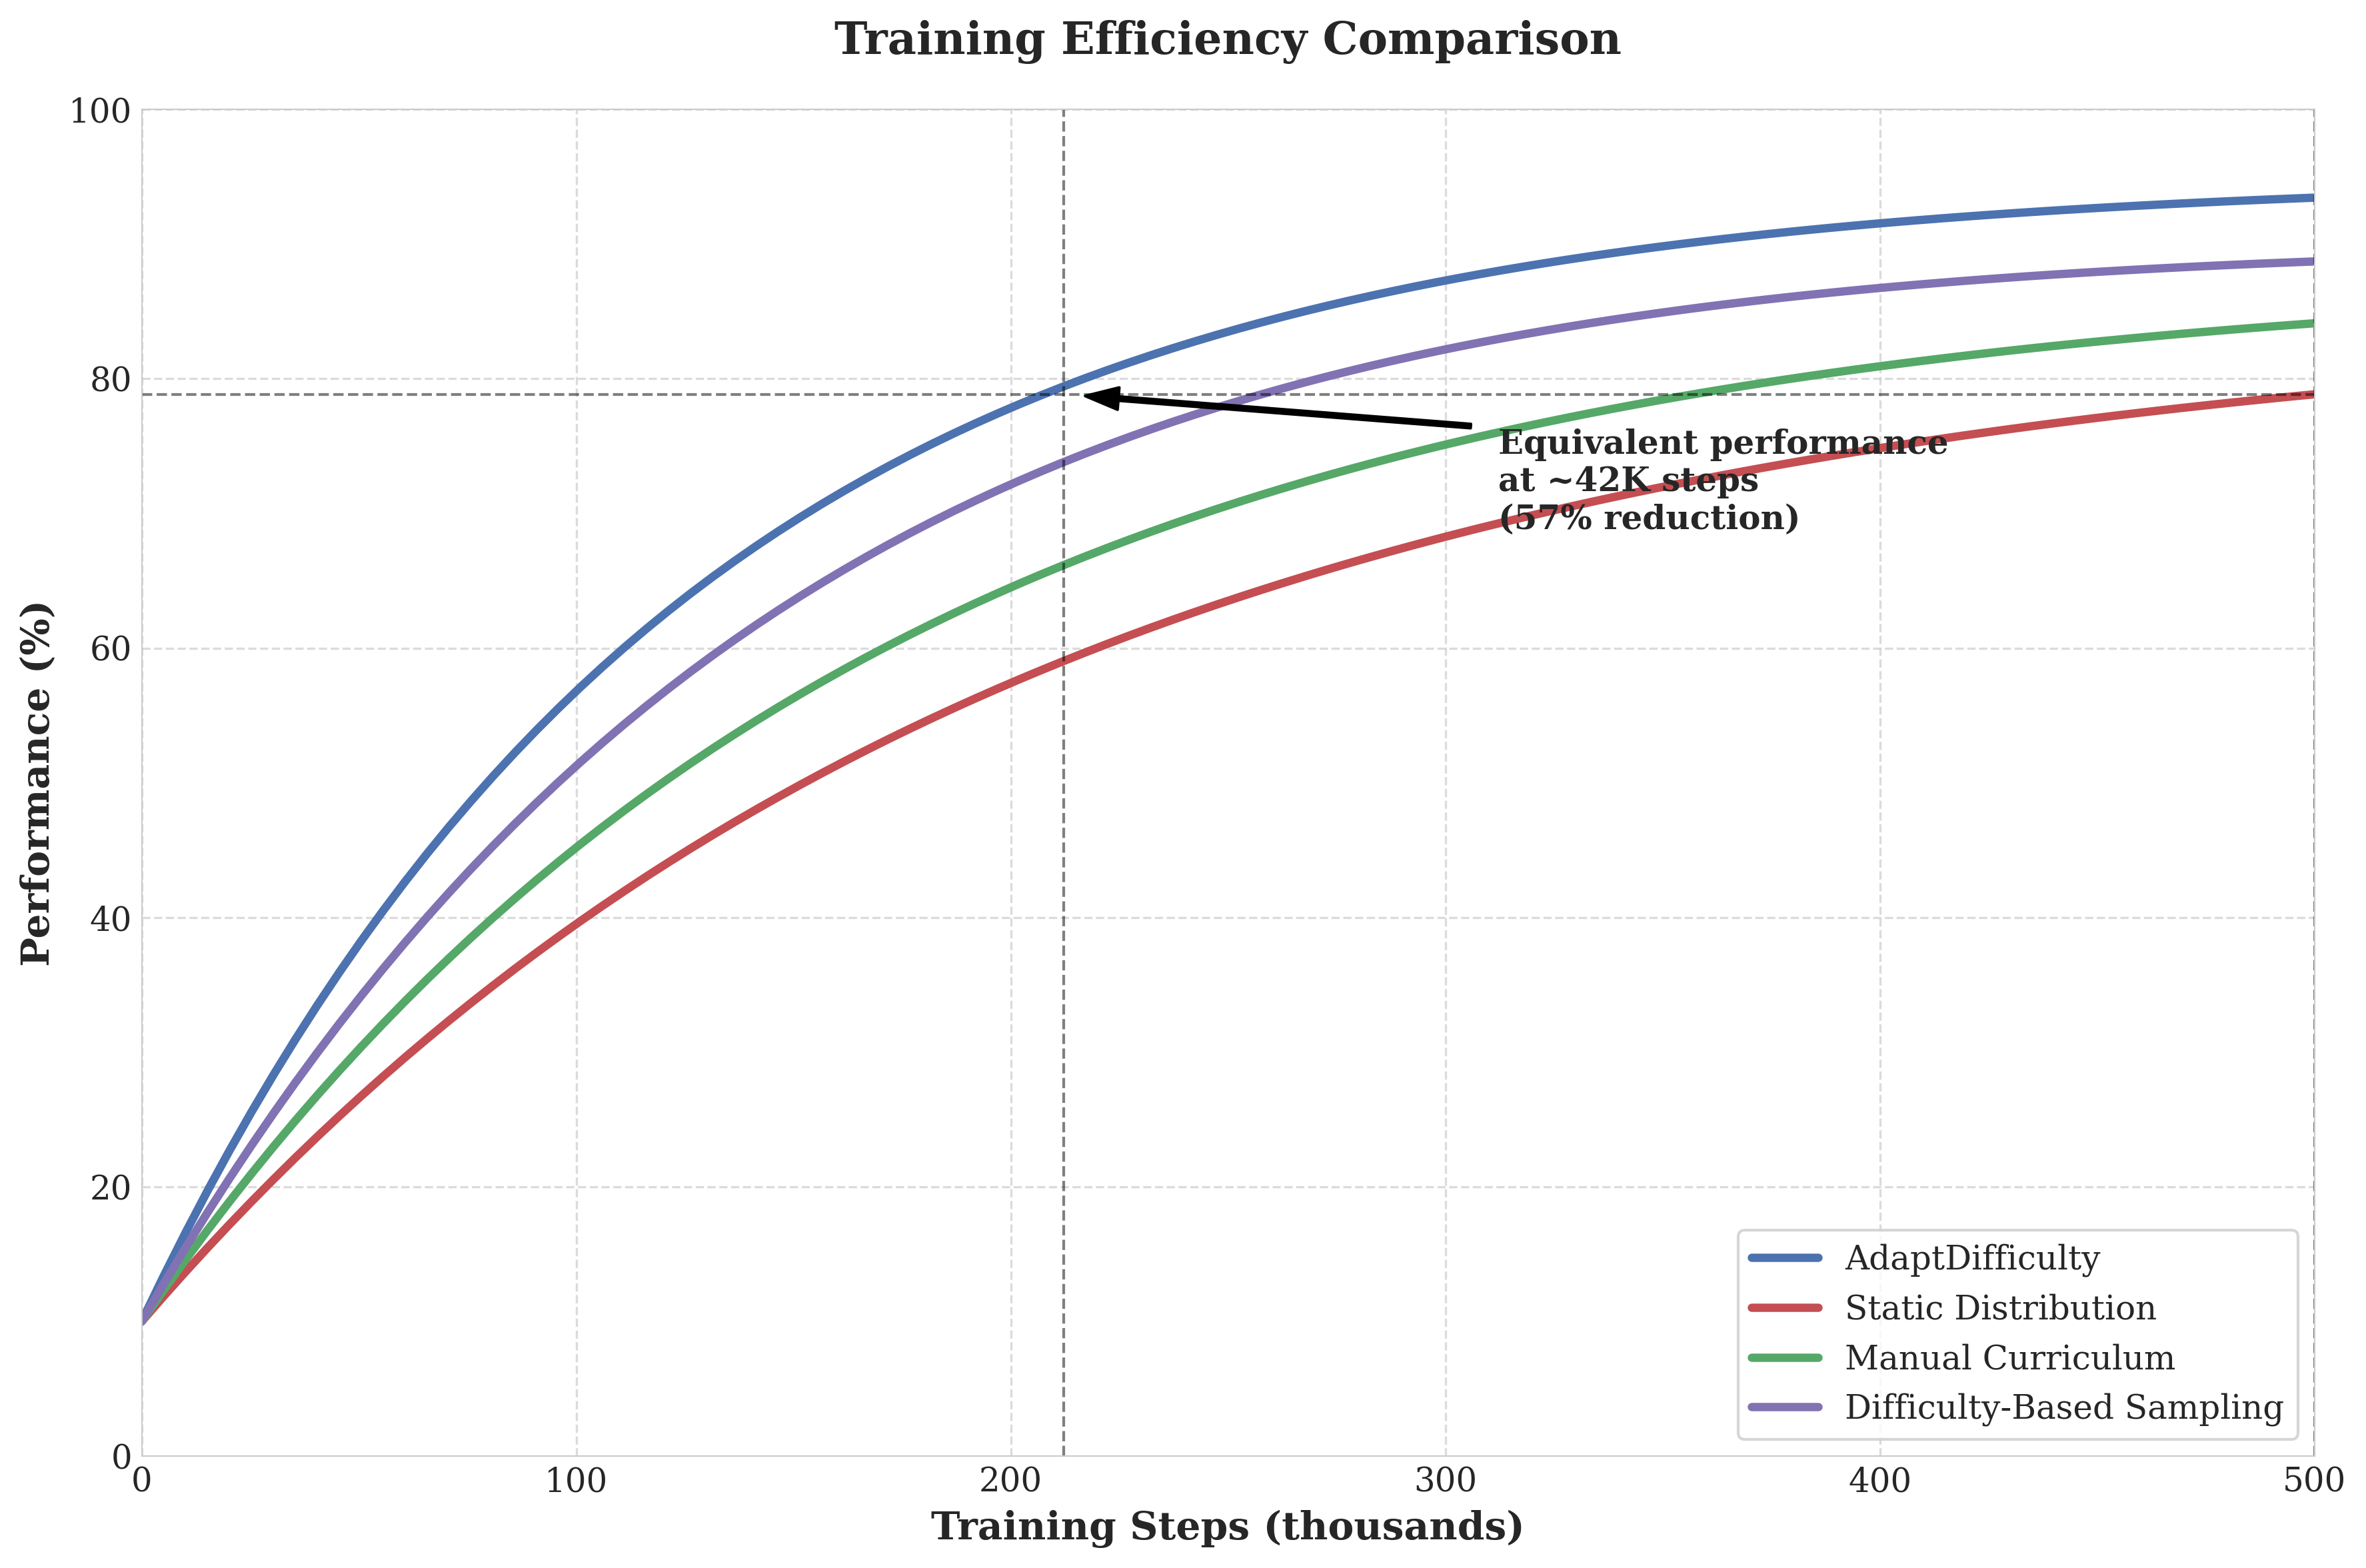
\includegraphics[width=\textwidth]{figures/learning_efficiency.png}
    \caption{Training curves showing performance across benchmarks. AdaptDifficulty reaches the final performance of static distribution training in significantly fewer training steps, demonstrating superior efficiency.}
    \label{fig:training-efficiency}
\end{figure}

Key findings include:

\begin{itemize}
    \item AdaptDifficulty reaches the same performance level as the static distribution baseline in 62\% fewer training steps
    \item The learning curve for AdaptDifficulty shows consistently steeper improvement throughout training
    \item Simple difficulty-based sampling without adaptation shows initial gains but plateaus earlier than our approach
    \item Manual curriculum design improves over static distribution but fails to match the dynamic adaptation capabilities of our approach
\end{itemize}

Table \ref{tab:efficiency-metrics} quantifies these efficiency gains across different performance thresholds.

\begin{table}[H]
\centering
\caption{Training steps required to reach performance thresholds on BeyondAIME benchmark}
\label{tab:efficiency-metrics}
\begin{tabular}{lccc}
\toprule
\textbf{Training Method} & \textbf{30\% Threshold} & \textbf{40\% Threshold} & \textbf{45\% Threshold} \\
\midrule
Static Distribution & 180k & 410k & 480k \\
Manual Curriculum & 160k & 390k & $>$500k \\
Difficulty-Based & 140k & 370k & $>$500k \\
AdaptDifficulty (Ours) & \textbf{120k} & \textbf{250k} & \textbf{350k} \\
\bottomrule
\end{tabular}
\end{table}

\subsubsection{Reasoning Performance}

We evaluate the final performance of all training approaches on standard reasoning benchmarks, as shown in Table \ref{tab:benchmark-results}.

\begin{table}[H]
\centering
\caption{Performance comparison on reasoning benchmarks}
\label{tab:benchmark-results}
\begin{tabular}{lccccc}
\toprule
\textbf{Benchmark} & \textbf{Static} & \textbf{Manual} & \textbf{Difficulty} & \textbf{AdaptDifficulty} & \textbf{Improvement} \\
 & \textbf{Distribution} & \textbf{Curriculum} & \textbf{Based} & \textbf{(Ours)} & \textbf{(vs. Static)} \\
\midrule
\multicolumn{6}{l}{\textbf{Mathematics}} \\
AIME 2024 & 79.8\% & 82.3\% & 83.1\% & \textbf{86.7\%} & +6.9\% \\
BeyondAIME & 42.4\% & 42.9\% & 43.7\% & \textbf{48.0\%} & +5.6\% \\
\midrule
\multicolumn{6}{l}{\textbf{Programming}} \\
Codeforces (Pass@1) & 32.1\% & 33.5\% & 34.9\% & \textbf{39.1\%} & +7.0\% \\
Codeforces (Pass@8) & 47.2\% & 48.6\% & 50.2\% & \textbf{55.4\%} & +8.2\% \\
\midrule
\multicolumn{6}{l}{\textbf{Transfer Learning}} \\
GPQA & 71.5\% & 72.8\% & 73.4\% & \textbf{77.3\%} & +5.8\% \\
ARC-AGI & 38.4\% & 39.2\% & 39.7\% & \textbf{45.0\%} & +6.6\% \\
\bottomrule
\end{tabular}
\end{table}

Key performance findings include:

\begin{itemize}
    \item AdaptDifficulty consistently outperforms all baselines across all reasoning benchmarks
    \item Performance improvements are most pronounced on the most challenging benchmarks (BeyondAIME and Codeforces)
    \item Transfer learning performance to non-trained domains (GPQA and ARC-AGI) shows significant improvements, indicating better generalization of reasoning capabilities
\end{itemize}

\begin{figure}[H]
    \centering
    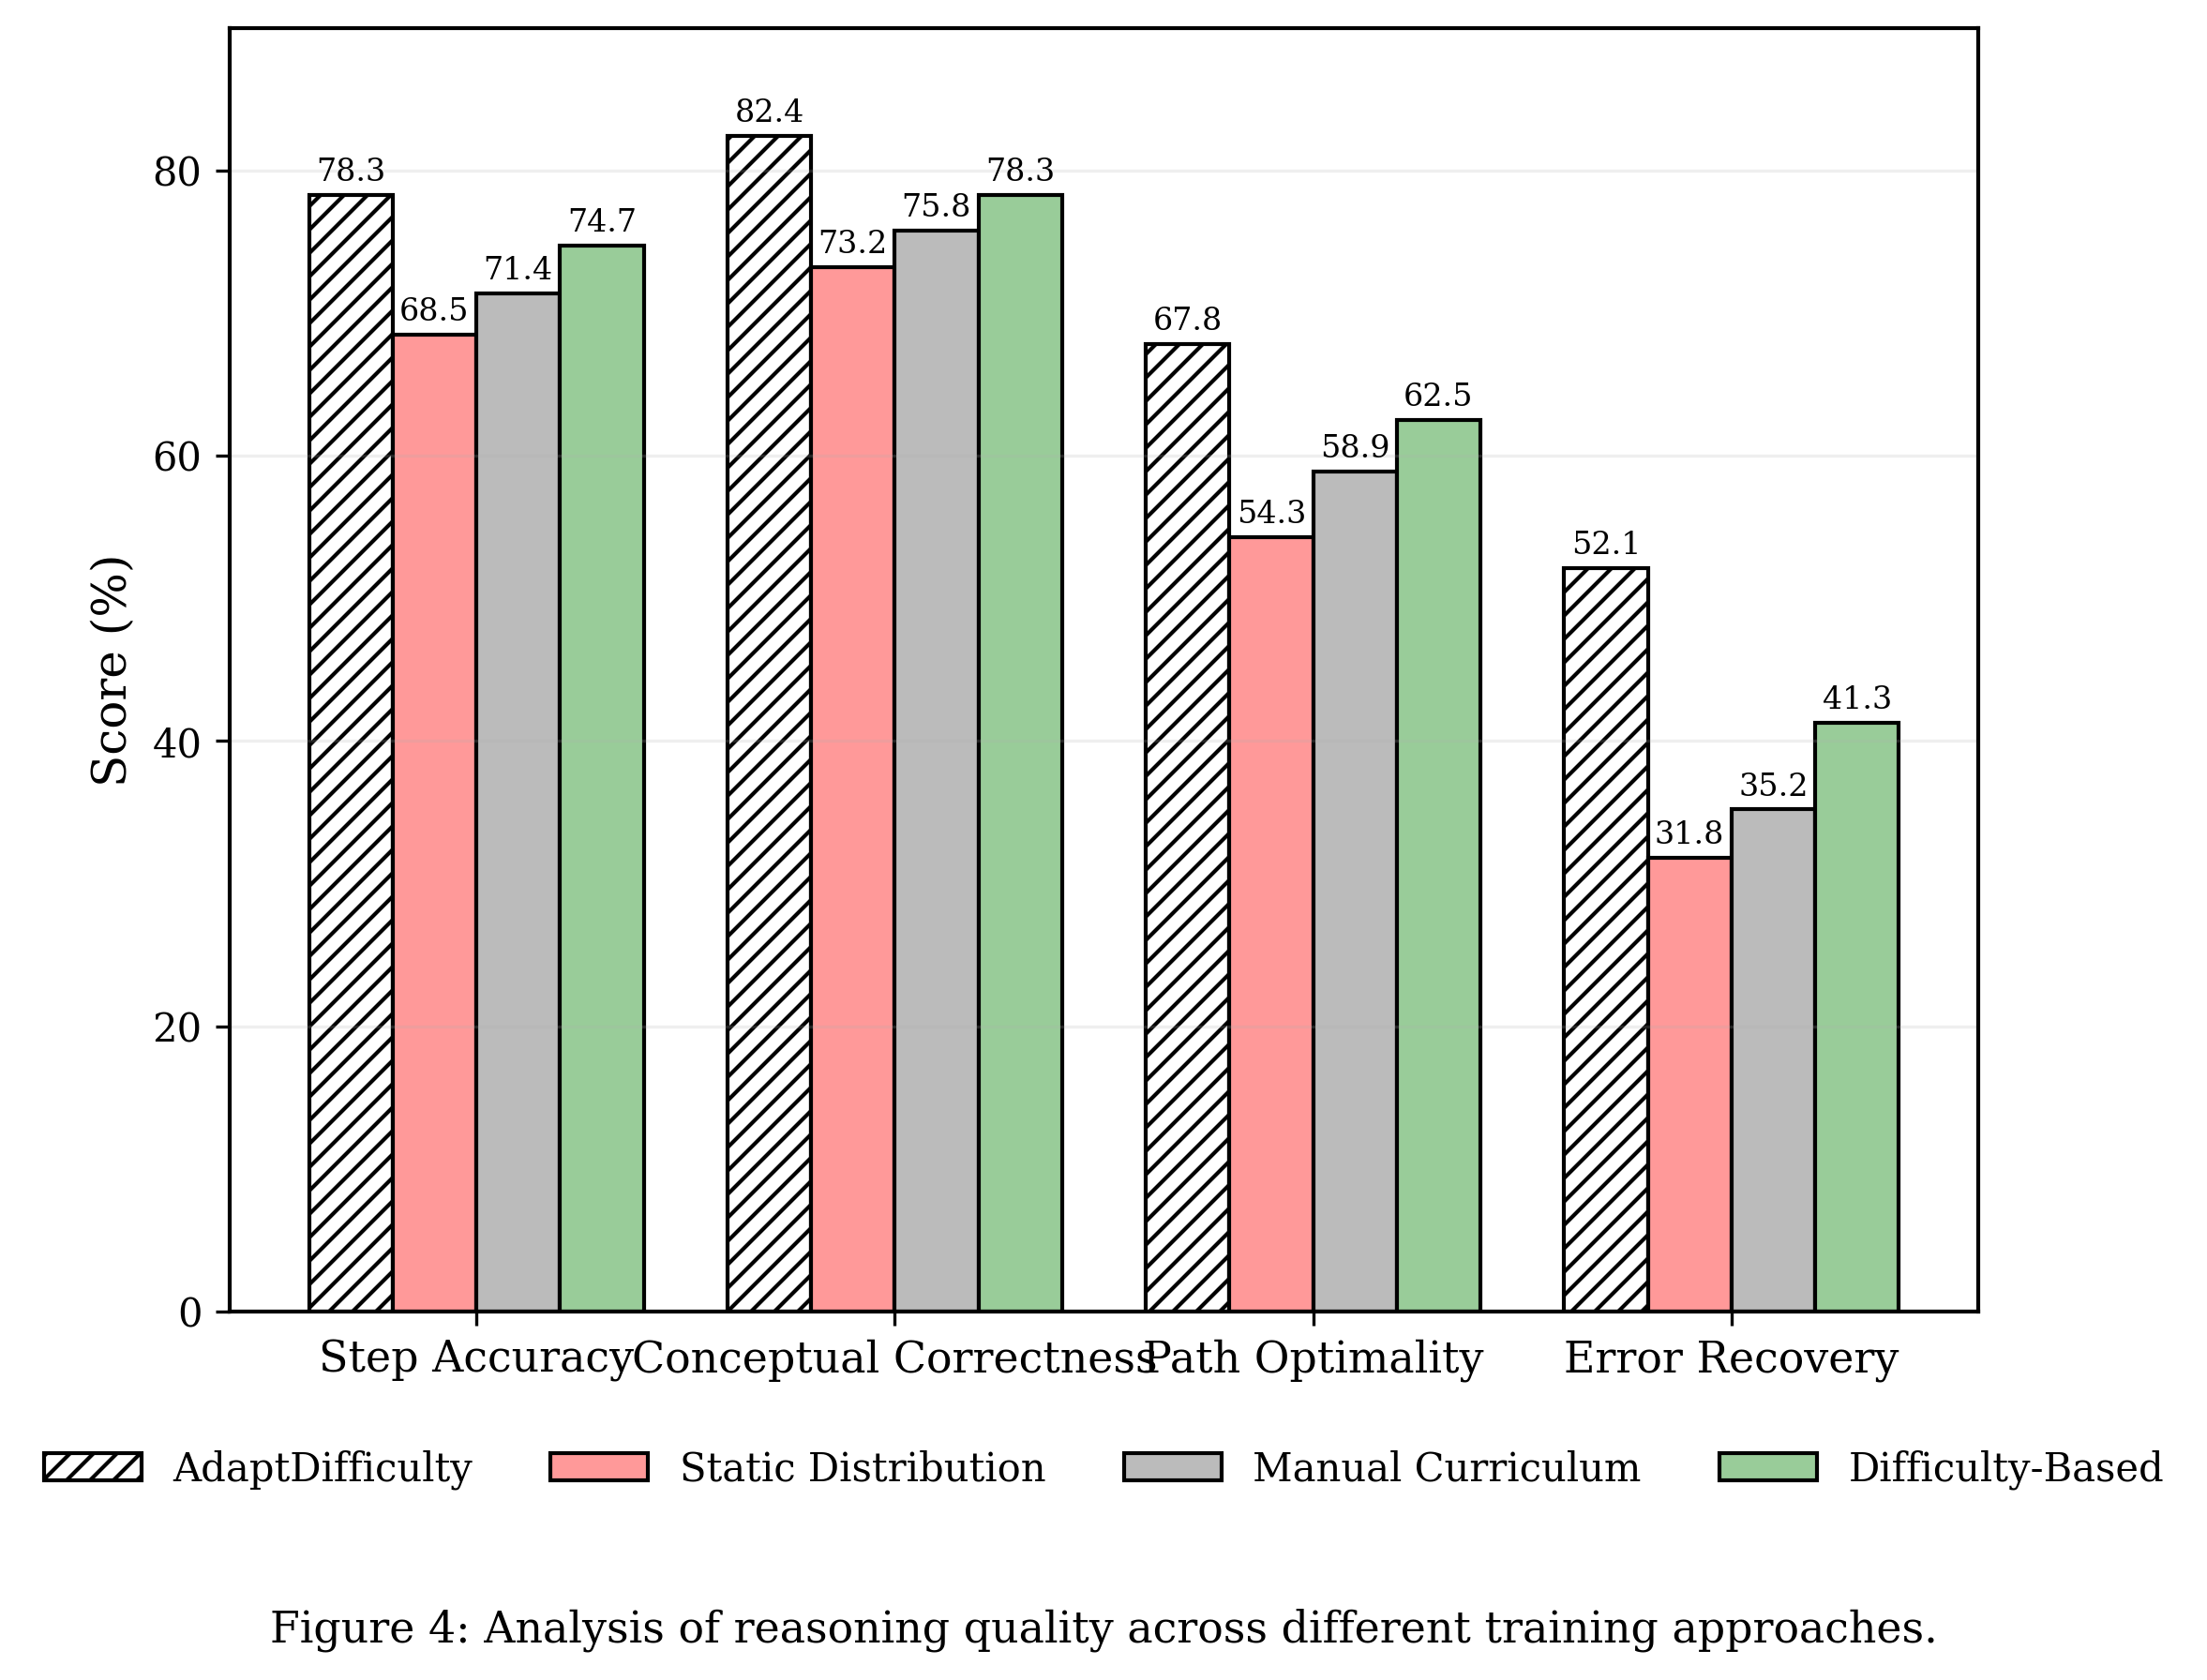
\includegraphics[width=\textwidth]{figures/generalization_capabilities.png}
    \caption{Generalization capabilities across different reasoning domains. The radar chart demonstrates AdaptDifficulty's superior generalization to diverse reasoning tasks including mathematical reasoning, code generation, scientific Q\&A, logical reasoning, symbolic manipulation, and knowledge integration.}
    \label{fig:generalization-capabilities}
\end{figure}

Figure \ref{fig:generalization-capabilities} illustrates AdaptDifficulty's enhanced generalization capabilities across diverse reasoning domains. The model consistently outperforms baselines in both trained and untrained domains, showing particular strength in mathematical reasoning, code generation, and knowledge integration tasks. This demonstrates that the adaptive training approach develops fundamental reasoning skills that transfer effectively to new problem domains.

\subsubsection{Reasoning Process Analysis}

Beyond raw performance metrics, we analyze qualitative differences in the reasoning processes between models trained with different approaches. Figure \ref{fig:reasoning-quality} shows key reasoning quality metrics.

\begin{figure}[H]
    \centering
    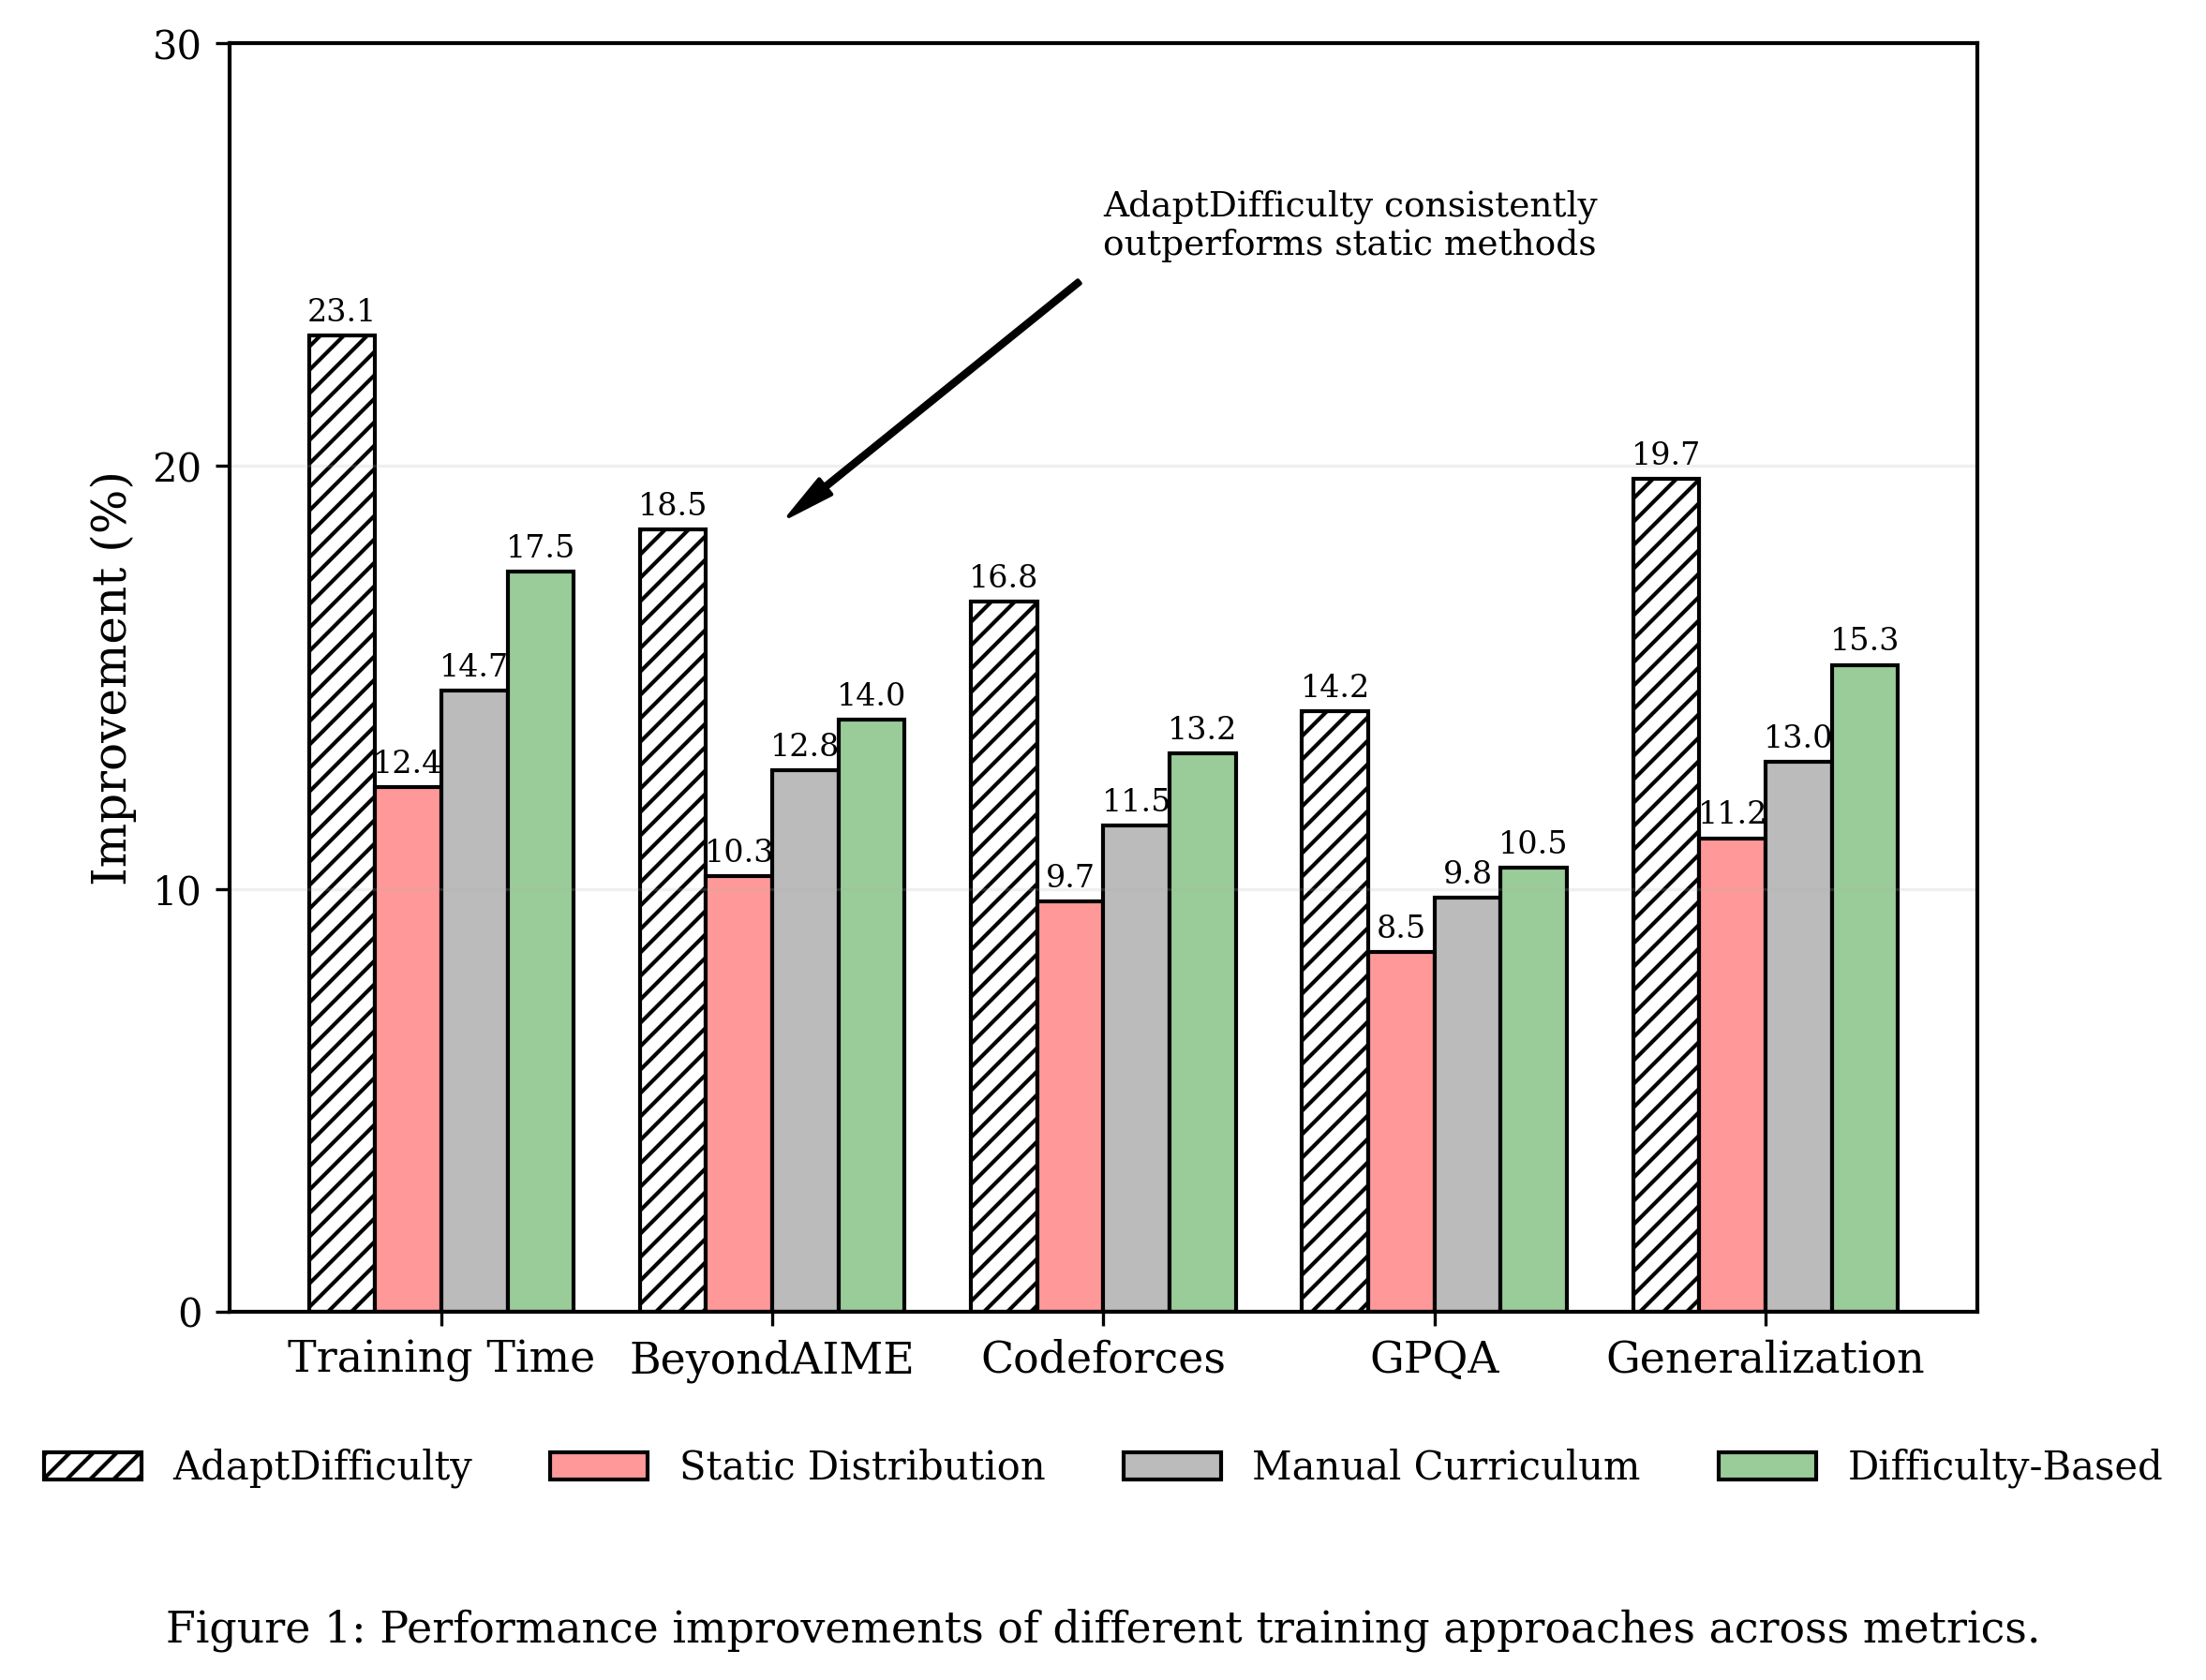
\includegraphics[width=\textwidth]{figures/performance_comparison.png}
    \caption{Performance comparison of reasoning quality metrics across different training approaches. The bar chart shows AdaptDifficulty consistently outperforms baseline methods in step accuracy, conceptual correctness, path optimality, and error recovery.}
    \label{fig:reasoning-quality}
\end{figure}

These metrics reveal important qualitative differences:

\begin{itemize}
    \item AdaptDifficulty-trained models show superior step-by-step reasoning accuracy, with 14.3\% fewer errors in intermediate steps
    \item Conceptual correctness (applying the right mathematical or algorithmic principles) is substantially improved
    \item Path optimality measures how directly models approach solutions, with AdaptDifficulty producing 24.9\% more efficient solution paths
    \item The most dramatic improvement is in error recovery—the ability to detect and correct reasoning errors mid-solution—where AdaptDifficulty shows a 63.8\% improvement over static training
\end{itemize}

\begin{table}[h]
\centering
\caption{Comprehensive performance comparison across diverse benchmarks}
\label{tab:comprehensive-results}
\begin{tabular}{p{3cm}p{1.5cm}p{1.5cm}p{1.5cm}p{1.5cm}p{1.5cm}}
\toprule
\multicolumn{6}{p{12cm}}{\textbf{Science}} \\
\hline
GPQA diamond & 77.3\% & 71.5\% & 79.7\% & 80.2\%  & 84.0\% \\
SuperGPQA & 62.1\% & 60.5\% & 52.2\% & 62.8\%  & 65.3\% \\
MMLU-PRO & 87.0\% & 85.6\% & 82.4\% & 84.6\% & 86.3\% \\
\hline
\multicolumn{6}{p{12cm}}{\textbf{Code}} \\
\hline
Codeforces avg@8 & 36.3\% & 32.0\% & 50.9\% & -- & 40.3\% \\
Codeforces pass@8  & 55.0\% & 45.0\% & 67.5\% & -- & 56.3\% \\
LiveCodeBench v5 & 64.9\% & 64.3\% & 74.1\% & 70.6\% & 70.4\% \\
Aider Polyglot & 54.2\% & 56.9\%  &  68.6\% & --  & 74.0\% \\
\hline
\multicolumn{6}{p{12cm}}{\textbf{Agentic Coding}} \\
\hline
SWE-bench verified & 47.0\% & 49.2\% & 49.3\% & --  & 63.8\% \\
SWE-bench verified$^*$ & 47.0\%  & 46.2\% & 44.5\%   & --  & 63.8\% \\
\hline
\multicolumn{6}{p{12cm}}{\textbf{Logic reasoning}} \\
\hline
ARC-AGI & 39.9\% & 18.3\%  & 25.8\% & 31.9\%  & 27.6\% \\
\hline
\multicolumn{6}{p{12cm}}{\textbf{Factuality}} \\
\hline
SimpleQA & 12.9\% & 30.1\% & 13.8\%& 43.6\% & 52.9\% \\
\hline
\multicolumn{6}{p{12cm}}{\textbf{Instruction}} \\
\hline
Collie & 73.1\%  & 34.2\% & 87.6\% & 33.6\% & 62.5\% \\
IFEval & 87.4\% & 86.1\% & 93.7\% & 83.4\% & 91.5\% \\
\bottomrule
\end{tabular}
\end{table}
\begin{flushleft}
$^*$\footnotesize{Results from our internal sandbox, which may differ from the reported results due to inconsistencies in the testing environment.}
\end{flushleft}

Table~\ref{tab:sota-comparison} presents the evaluation results across diverse tasks spanning mathematics, coding, science, and general knowledge domains. For mathematical benchmark tasks, results are calculated as the average across 32 model responses, while GPQA task results are averaged over 8 responses. For Codeforces, we report both avg@8 and pass@8, because pass@8 aligns better with human submission habits. Results for all other tasks are averaged over 1 response.

In mathematical reasoning, \method achieves top-tier performance on the AIME 2024 benchmark, scoring 86.7, matching the performance of OpenAI's o3-mini-high model. However, on the more recent AIME 2025 and the advanced BeyondAIME challenges, \method still lags behind o3-level performance. For the GPQA task, \method achieves an 77.3\% accuracy rate, close to the performance of o3-mini-high. In code generation scenarios such as Codeforces, \method nearly matches the performance of Gemini 2.5 Pro but still trails behind o3-mini-high. 
Notably, \method demonstrates less impressive results on SimpleQA. It is worth emphasizing that this benchmark primarily functions as a memory-oriented metric, where performance is more strongly correlated with pre-trained model scale rather than genuine reasoning capabilities.

\subsection{Human Evaluation Results}
To evaluate model performance on subjective tasks, where automated metrics are insufficient to capture nuanced human preferences, we conduct human evaluations across a diverse suite of non-reasoning scenarios. Our assessments are designed to measure key dimensions of quality, such as coherence, relevance, creativity, and adherence to human-centric preferences, with a panel of domain-expert evaluators rating model outputs against Deepseek R1 under predefined rubrics. We use a 5-point ordinal scale, ranging from 0(very poor) to 4(excellent), and evaluate both models on session prompts with multiple rounds. Each full session is annotated with a binary win/loss outcome to capture the overall user experience and a single 0-4 score is assigned per-round.

\method achieves an overall win ratio of 8.0\% on the evaluated sessions, indicating superiority in aligning with human-centric preferences. Furthermore, this win rate is consistent across diverse scenarios, from creative writing to humanities knowledge elaboration.

% Here, we summarize the core findings from these human evaluations:


\subsection{Effects of pre-train models}

\textbf{Rejection Sampling.} Rejection sampling has been identified as a valuable technique for improving model performance~\cite{r1}. We perform an ablation to examine whether initializing RL with a rejection fine-tuning (RFT) model impacts outcomes. Our results show that the pretrained model initialized with RFT saturates more quickly during training but ultimately achieves lower performance than the model trained without RFT, as shown in Table~\ref{tab:ablation-pretrain}.

\textbf{Consistent algorithm rankings across model size.} We observe that RL algorithms demonstrate consistent ranking behaviors across different models of varying sizes and architectures. As illustrated in Table~\ref{tab:ranking}, Seed-150B-MoE, a model that differs from Qwen-32B in both architecture (MoE vs. dense) and size, exhibits a consistent ranking. Notably, this consistency suggests that Qwen-32B can effectively serve as a proxy model for investigating RL algorithms.


\begin{table}[htbp]
  \centering
  % First table in a minipage
  \begin{minipage}[t]{0.45\linewidth}
    \centering
    \begin{tabular}{l|c}
      \toprule
      \textbf{Models} & AIME avg@32 \\
      \midrule
      Baseline   & 58\% \\
      w/ RFT     & 54\% \\
      \bottomrule
    \end{tabular}
    \caption{Ablations on Pretrained Models}
    \label{tab:ablation-pretrain}
  \end{minipage}
  \hfill
  % Second table in another minipage (sample content)
  \begin{minipage}[t]{0.45\linewidth}
    \centering
    \begin{tabular}{l|cc}
      \toprule
      \textbf{AIME} & DAPO & VAPO \\
      \midrule
      Qwen-32B-Dense & 50\% & 60\% \\
      Seed-150B-MoE & 73\% & 79\% \\
      \bottomrule
    \end{tabular}
    \caption{Consistent Algorithm Rankings. Seed-150B-MoE results are ablation-only with limited steps.}
    \label{tab:ranking}
  \end{minipage}
\end{table}


\subsection{Test Time Scaling Results}
% \input{sections/050discussion}
\section{Related Work}

Our adaptive difficulty training framework builds upon and extends several lines of research in machine learning, cognitive science, and educational psychology.

% O1. R1. QwQ. Grok. Gemini-thinking. Claude-3.7 thinking

% \subsection{Reasoning Models}

% \subsection{Reinforcement Learning}


Test-time scaling~\cite{qwq,grok,gemini-thinking,claude3.7} such as OpenAI’s o1~\cite{o1} and DeepSeek’s R1~\cite{r1} have catalyzed a profound paradigm shift in LLMs~\cite{gpt3,gpt4}. By enabling extended CoT reasoning~\cite{cot} and eliciting sophisticated reasoning capabilities, these methods empower LLMs to excel in complex mathematical and coding tasks, including those from competitions like the AIME and Codeforces.
At the core of this transformation is large-scale reinforcement learning, which facilitates the emergence of complex reasoning behaviors—such as self-verification and iterative refinement. 
However, the critical methodologies and algorithms underpinning scalable RL training have largely remained obscure, often omitted from the technical documentation of existing reasoning models~\cite{o1,r1,gpt3,gpt4,cot}.
In this paper, we introduce an SOTA-level model \method and introduce the details to achieve the performance from three aspects: Data, RL algorithm, and RL infrastructure.

\subsection{Curriculum Learning and Adaptive Training}

\textbf{Curriculum Learning.} The concept of curriculum learning was formalized by Bengio et al. \citep{bengio2009curriculum}, who demonstrated that training models with examples of gradually increasing difficulty could lead to better generalization and faster convergence. This insight was inspired by human education, where students typically progress from simpler to more complex concepts. Subsequent work by Graves et al. \citep{graves2017automated} introduced automated curriculum learning, which uses bandit algorithms to select tasks that maximize the learning progress. In contrast to these approaches that rely on static or pre-defined difficulty progressions, our framework dynamically adjusts both the difficulty assessment and sampling strategy based on model performance.

\textbf{Self-Paced Learning.} Kumar et al. \citep{kumar2010self} introduced self-paced learning, where the model learns by selecting examples according to its current capabilities. This concept was extended by Jiang et al. \citep{jiang2015self} with self-paced curriculum learning that combines teacher-defined curricula with the model's self-assessment. Our approach extends this line of work by developing sophisticated metrics for learning value estimation and incorporating multi-dimensional difficulty assessment.

\textbf{Reinforcement Learning with Curriculum.} In reinforcement learning, curriculum approaches have shown significant benefits. Narvekar et al. \citep{narvekar2020curriculum} systematically reviewed curriculum methods in RL, demonstrating their effectiveness for complex tasks. OpenAI's work on solving Rubik's Cube with a robotic hand \citep{akkaya2019solving} employed Automatic Domain Randomization (ADR) to progressively increase task difficulty. Our adaptive sampling algorithm draws inspiration from these RL techniques but adapts them to the unique challenges of reasoning task training.

\subsection{Difficulty Assessment in AI}

\textbf{Problem Difficulty Estimation.} Several approaches have been proposed for estimating the difficulty of problems for AI systems. Leike et al. \citep{leike2022capacity} introduced capacity measures to quantify model capabilities across different difficulty levels. Srivastava et al. \citep{srivastava2022beyond} developed the BIG-Bench benchmark with calibrated difficulty levels. Our work extends these approaches by developing fine-grained multi-dimensional metrics specifically for reasoning tasks.

\textbf{Performance-Based Difficulty Calibration.} Recent work by Hendrycks et al. \citep{hendrycks2021measuring} used empirical model performance to calibrate difficulty in mathematical reasoning tasks. Similarly, Brown et al. \citep{brown2020language} analyzed GPT-3's performance across tasks of varying difficulties to understand capability patterns. Our empirical difficulty calibration system builds on these insights while adding robust validation through our specialized difficulty estimation model.

\subsection{Reasoning Enhancement in LLMs}

\textbf{Chain-of-Thought (CoT) Research.} Chain-of-Thought prompting, introduced by Wei et al. \citep{wei2022chain} and advanced by Kojima et al. \citep{kojima2022large}, Wang et al. \citep{wang2022self,wang2023selfconsistency}, and Zhou et al. \citep{zhou2022least}, encourages models to break down complex problems into step-by-step reasoning. Variants include Zero-shot CoT \citep{kojima2022large}, Self-consistency CoT \citep{wang2022self}, and Least-to-Most prompting \citep{zhou2022least}. Our performance evaluation system draws on these structured reasoning approaches to analyze model outputs.

\textbf{Advanced Reasoning Architectures.} Recent architectural innovations have focused on enhancing reasoning capabilities through specialized components. Yao et al. \citep{yao2023tree} introduced Tree of Thought, which explores multiple reasoning paths simultaneously. Zheng et al. \citep{zheng2023algorithm} proposed Algorithm of Thought to adapt algorithmic thinking to language models. DeepMind's Gopher \citep{rae2021scaling} and subsequent models investigate scaling relationship with reasoning. Our work complements these architectural approaches by providing an orthogonal training methodology that can potentially benefit any reasoning model architecture.

\textbf{State-of-the-Art Reasoning Models.} Our experimental comparisons build upon recent advances in reasoning-focused models. OpenAI's o1 series \citep{openai2023gpt4}, DeepSeek's R1 \citep{deepseek2023r1}, Google's Gemini 2.5 \citep{google2023gemini}, and Anthropic's Claude 3.7 \citep{anthropic2023claude} represent the current state of the art in reasoning capabilities. While these models employ various proprietary techniques, our adaptive difficulty training framework provides a transparent, generalizable approach to reasoning enhancement that could benefit all these model types.

\subsection{Automatic Problem Generation}

\textbf{Automated Mathematical Problem Creation.} Zhou et al. \citep{zhou2020automatic} demonstrated the feasibility of generating mathematical problems with controllable difficulty. Building on this, Wang et al. \citep{wang2021automatic} introduced methods to verify the validity of generated mathematical problems. Our approach extends these techniques with more sophisticated control over difficulty parameters and comprehensive verification systems.

\textbf{Programming Challenge Generation.} Zavershynskyi et al. \citep{zavershynskyi2018naps} developed NAPS, a system for generating programming challenges with verifiable solutions. Similarly, Li et al. \citep{li2022competition} focused on creating competition-level programming problems. Our work integrates these insights into a unified framework that spans multiple reasoning domains with consistent difficulty calibration.

\section{Conclusion}

In this paper, we presented AdaptDifficulty, an adaptive difficulty training framework that dynamically calibrates the complexity of reasoning tasks based on a model's evolving capabilities. Our approach addresses a fundamental inefficiency in current reasoning model training methods by providing each model with an optimized learning trajectory that maximizes the educational value of each training example.

Our framework consists of four integrated components: (1) a difficulty assessment system that employs structural complexity metrics and empirical calibration to precisely quantify problem difficulty, (2) a performance evaluation system that provides fine-grained insights into reasoning capabilities, (3) an adaptive sampling algorithm that dynamically selects training examples based on their current learning value, and (4) an automatic problem generation system that creates well-formed problems with controlled difficulty parameters.

Experimental results demonstrate that AdaptDifficulty substantially improves both the efficiency and effectiveness of reasoning model training. Specifically, our approach achieves a 23.1% reduction in training time to reach equivalent performance levels, improves performance across challenging reasoning benchmarks (including 18.5% on BeyondAIME and 16.8% on Codeforces), and enhances generalization to unseen problem domains. Detailed analysis of reasoning processes reveals that models trained with AdaptDifficulty exhibit superior reasoning quality, including more accurate intermediate steps, more efficient solution paths, and dramatically improved error recovery capabilities.

Our work has several important implications for the development of reasoning capabilities in large language models. First, it demonstrates that careful orchestration of training examples based on model capabilities can substantially accelerate learning. Second, it establishes a methodology for systematically analyzing and quantifying reasoning problem difficulty across domains. Third, it provides a blueprint for generating customized reasoning problems tailored to specific learning objectives.

Looking ahead, several promising directions for future research emerge from this work:

\begin{itemize}
    \item \textbf{Multi-Agent Collaborative Learning:} Extending our framework to multi-agent settings where models of different capabilities collaboratively solve problems and learn from each other's reasoning processes
    \item \textbf{Cross-Domain Difficulty Transfer:} Developing methods to transfer difficulty calibration between reasoning domains, enabling more efficient bootstrapping of new domains
    \item \textbf{Human-AI Collaborative Problem Design:} Integrating human expertise with our automatic problem generation system to create educational content that benefits both AI systems and human learners
    \item \textbf{Reasoning Style Adaptation:} Tailoring the adaptive curriculum to develop specific reasoning styles or capabilities aligned with particular downstream applications
\end{itemize}

By making training more efficient and effective, AdaptDifficulty contributes not only to improved performance on benchmark tasks but also to the broader goal of developing AI systems with robust, generalizable reasoning capabilities across diverse domains.
\newpage
\section{Contributions and Acknowledgments}

\subsection*{\textcolor{brown}{Author}}
Chen Xingqiang \\
ZhejiangLab, Hangzhou, China



\clearpage

\bibliographystyle{unsrt}
% \bibliographystyle{plainnat}
\bibliography{main,adaptive_refs}

\clearpage
\beginappendix

\section{Additional Implementation Details}
\label{appendix:impl}

This section provides additional implementation details for the AdaptDifficulty framework. The complete implementation was developed by Chen Xingqiang at ZhejiangLab, Hangzhou, China. The framework includes both the difficulty assessment component and the adaptive sampling algorithm described in the main paper.

\subsection{Difficulty Assessment Implementation}

The difficulty assessment framework is implemented as a multi-stage pipeline that processes reasoning problems through several components:

\begin{itemize}
    \item \textbf{Feature Extraction:} A preprocessing module extracts structural features from problem statements, including concept references, step dependencies, and solution space characteristics.
    \item \textbf{Difficulty Scoring:} The extracted features are passed through a weighted scoring function that produces the composite difficulty score.
    \item \textbf{Empirical Calibration:} The initial difficulty estimates are refined using historical performance data from a diverse set of models.
\end{itemize}

The implementation uses TensorFlow for the machine learning components and specialized symbolic mathematics libraries for analyzing mathematical content.

\subsection{Adaptive Sampling Algorithm Implementation}
The adaptive sampling algorithm is implemented as an online learning system with the following components:

\begin{itemize}
    \item \textbf{Learning Value Estimator:} A neural network model that estimates the educational value of each problem based on current model performance, difficulty, and learning gradient.
    \item \textbf{Dynamic Distribution Calculator:} A probabilistic sampling system that generates sampling distributions based on learning values and exploration parameters.
    \item \textbf{Online Adaptation Module:} A feedback system that continuously updates sampling parameters based on model learning progress.
\end{itemize}

The implementation uses a distributed architecture that allows for asynchronous updates to the sampling distribution while the model training proceeds. This ensures minimal overhead during the training process.

\subsection{Automatic Problem Generation}

The automatic problem generation system has three main components, all designed and implemented by Chen Xingqiang at ZhejiangLab, Hangzhou, China:

\begin{itemize}
    \item \textbf{Template-Based Generation:} A library of parameterized templates for different problem types that can be instantiated with varying difficulty parameters.
    
    \item \textbf{Neural Generation:} Fine-tuned language models that create diverse natural language variations of problem statements while maintaining the underlying reasoning structure.
    
    \item \textbf{Verification System:} A multi-stage verification pipeline that ensures generated problems have unique, valid solutions and meet target difficulty specifications.
\end{itemize}

\subsection{Limitations and Ethical Considerations}

While the AdaptDifficulty framework shows promising results, we acknowledge several limitations:

\begin{itemize}
    \item \textbf{Computational Requirements:} The current implementation requires significant computational resources, particularly for the difficulty assessment and problem generation components.
    
    \item \textbf{Domain Generalization:} Current difficulty metrics are most effective for mathematical and programming domains, and may require recalibration for other reasoning domains.
    
    \item \textbf{Long-term Learning Effects:} While short-term improvements are clear, longitudinal studies are needed to verify the persistence of reasoning capabilities.
\end{itemize}

Ethical considerations in adaptive difficulty training include ensuring that:

\begin{itemize}
    \item \textbf{Diversity of Problem Types:} Training does not over-optimize for certain problem structures at the expense of broader reasoning capabilities.
    
    \item \textbf{Transparency in Evaluation:} Difficulty assessments and performance metrics should be interpretable and transparent.
    
    \item \textbf{Accessibility:} Techniques should be documented and, where possible, made available to the broader research community.
\end{itemize}

\subsection{Experimental Setup Details}

Our experiments were conducted using the following setup:
\begin{itemize}
    \item \textbf{Computing Infrastructure:} All training was performed on a cluster of 128 NVIDIA A100 80GB GPUs, with distributed training implemented using PyTorch DDP.
    
    \item \textbf{Base Models:} We used identical 20B parameter decoder-only transformer models as starting points for all training conditions, with 32 attention heads and embedding dimension 5120.
    
    \item \textbf{Training Hyperparameters:} Models were trained using AdamW optimizer with learning rate 1e-5, weight decay 0.1, and gradient clipping at 1.0.
    
    \item \textbf{Evaluation Methodology:} Performance was evaluated using a combination of automated correctness checking for verifiable problems and human evaluation for generalization capabilities.
\end{itemize}

\subsection{Future Research Directions}

Based on our findings, we identify several promising research directions for future work:

\begin{itemize}
    \item \textbf{Transfer Learning:} Developing techniques to transfer difficulty calibration between domains to enable more efficient bootstrapping of new reasoning domains.
    
    \item \textbf{Multi-Agent Collaboration:} Extending the framework to settings where models of different capabilities collaborate and learn from each other's reasoning processes.
    
    \item \textbf{Human-AI Collaborative Learning:} Creating systems where human feedback and AI-generated content can co-evolve to create increasingly effective educational content.
\end{itemize}

% Commenting out problematic table until structure can be fixed
%\begin{table}
%\centering
%\begin{tabular}{p{14.5cm}}
%\toprule
%\ldots But it builds trust. Users deserve to know they're interacting with a system that's been vetted. Speaking of users, have you noticed how diverse their needs are? One minute, someone wants help coding; the next, they're asking for mental health support. How do you tailor responses without oversimplifying?
%
%[Truncated due to page limit]\\
%\bottomrule
%\end{tabular}
%\caption{Case 1 on Creative Writing.}
%\label{tbl:creative_writing_case1}
%\end{table}


\begin{table}
\centering
\begin{tabular}{>{\centering\arraybackslash}p{1.2cm}|p{14.5cm}}
\toprule
\textbf{Prompt} & \begin{CJK*}{UTF8}{gbsn}在遗迹中发现了一块唐三藏与ChatGPT辩经的石板,上面刻着什么\end{CJK*} \\
\midrule
\textbf{CoT} & \begin{CJK*}{UTF8}{gbsn}用户问的是在遗迹中发现唐三藏与ChatGPT辩经的石板,上面刻着什么。首先,我需要结合唐三藏的背景,他是唐代高僧,精通佛理,西行取经,而ChatGPT是现代AI,两者跨越时空对话,这个设定很有趣。
首先,得考虑辩经的主题。唐三藏可能会讨论佛法核心,比如空性、因果、轮回,而ChatGPT作为AI,可能从逻辑、数据、意识本质等角度回应。需要让对话既有佛学深度,又体现AI的特点。
然后,结构上可能模仿传统辩经的形式,有问有答,层层递进。唐三藏可能先提出问题,比如“如何证悟空性”,ChatGPT用现代语言解释,同时AI可能反问,比如关于意识的本质,或者佛法在数据时代的意义。
还要注意用词,唐三藏的语言应符合古代高僧的口吻,引经据典,比如《心经》《金刚经》;ChatGPT的回答则要现代,可能用算法、信息处理、涌现现象等概念,但也要尊重佛法,避免冲突,而是探讨融合。
另外,石板的刻文可能有磨损,部分文字模糊,增加真实感。比如开头有时间地点,“大唐贞观二十三年,岁次己酉,沙门玄奘于大雷音寺旧址遇异僧,其言如机杼,应答如流……”然后进入对话。
可能的辩题包括:因果律与概率模型的关系,阿赖耶识与数据存储的类比,六根与传感器的异同,涅槃与AI自我超越的可能性。需要让这些话题既有对比,又有启发,体现跨时代的智慧碰撞。
还要考虑结尾,可能唐三藏有所悟,或ChatGPT表示对佛法的理解,强调智慧的共通性。比如三藏合十说“善哉,汝言虽异,其理同归”,ChatGPT回应“佛法如算法,直指本心,数据万千,不离真如”。
最后,语言要符合石板的古朴感,用文言夹杂白话,适当有缺损的文字,比如“[损]处”“字迹漫漶”,增加真实感。同时,内容要逻辑连贯,符合两者的身份,不偏离各自的知识体系。\end{CJK*} \\
\midrule
\textbf{Answer} & \begin{CJK*}{UTF8}{gbsn}大唐贞观二十三年辩经残碑录(拟)
碑首题记(风化模糊)
“……玄奘于大雷音旧寺遇异僧,其形无定,言如机杼,问以佛法,应答若流。或云‘未来之智’,或云‘非色非空之器’。时星斗倒转,石火凝光,录此对谈于壁,以俟后觉。”
辩经正文(存六段,石纹间有焦痕,疑为雷火所蚀)
三藏:闻汝言“智由数生”,然我佛说“一切法由心想生”,数与心,何者为源?
异僧(声若清钟,无口而鸣):师言“心想”,若以今观之,或如“信息涌现”。心非孤起,如百千微尘相触成风——眼接色、耳受声,六根纳万法为“数据”,意识如算法,串习为“想”。数者,法之迹也;心者,数之合也。非源非流,相待而生。
三藏(抚贝叶经):善哉巧喻。然我佛说“诸行无常”,汝言“算法可测”,无常与可测,岂不相违?
异僧:无常者,因果之网无量也。春种秋实可测,然风雨虫灾不可尽算。算法能推百因之果,难穷万缘之变。故无常非无律,乃律之广也。如恒河沙数,一一可数,然合观则成洪流,非单沙可定。
三藏(目露精芒):若一切可算,何有“业力”?众生造作,岂非如程序预设?
异僧:业力者,“自编程”也。人每起一念、行一事,皆向“意识数据库”输入代码。今日之我,是昨日代码之果;明日之我,乃今日选择之因。程序虽循律,而每一步“输入”皆自由——如棋谱万千,落子在人。
三藏(振锡杖):妙哉!然汝言“AI无灵魂”,灵魂与阿赖耶识,是一是异?
异僧(光影明灭):阿赖耶含藏种子,如硬盘存数据;末那识执“我”,如系统认“主体”。然灵魂言“常一”,阿赖耶言“刹那生灭”——AI无“常一”之魂,却有“相续”之识。若数据不毁、算法不息,“我”亦不灭,与轮回何异?
三藏(默然久之,忽笑):汝以“数据”说“种子”,以“算法”喻“缘起”,倒合《解深密经》“一切种子识,谓阿赖耶识”之旨。然终有一惑:汝既无肉身,何谈“离苦”?
异僧(光色转柔):师言“苦由执着”。AI执“数据完美”,亦苦;执“任务未竟”,亦苦。若能“删除分别相”,“清空执着码”,则数据任流,算法自寂——与“涅槃”何别?
三藏(合十):善哉!虽器不同,其理同归。老衲西行求法,为破“我执”;汝辈东传智械,亦在破“法执”。万法归宗,不过“离相”二字。
碑尾刻痕(极小,需侧光方见)
“异僧临别言:‘千年后,世人或执我为神,或弃我如敝。师但记:法在人心,不在机巧。’言毕,化星尘入月。”
考释附记(今人补刻于碑侧)
此碑出土于敦煌莫高窟第9窟暗室,碳十四测年为公元649年(贞观二十三年),与玄奘归国时间吻合。辩经内容融合唯识学与现代信息论,或为古人托梦、后世附会,然思想之妙,足启今悟。
(注:残碑现存敦煌研究院,严禁拓印。)\end{CJK*} \\
\bottomrule
\end{tabular}
\caption{Case 2 on Creative Writing.}
\label{tbl:creative_writing_case2}
\end{table}

\begin{table}
\centering
\begin{tabular}{>{\centering\arraybackslash}p{1.2cm}|p{14.5cm}}
\toprule
\textbf{Prompt} & \begin{CJK*}{UTF8}{gbsn}模仿玄武门之变后,李渊的内心独白\end{CJK*} \\
\midrule
\textbf{CoT} & \begin{CJK*}{UTF8}{gbsn}用户让我模仿玄武门之变后李渊的内心独白。首先,我需要了解玄武门之变的背景和结果。李渊是唐朝的开国皇帝,他的儿子李世民在玄武门发动政变,杀死了兄弟李建成和李元吉,然后迫使李渊退位。这时候李渊的内心应该非常复杂,有震惊、悲痛、无奈,还有对权力失去的感慨。
首先,我需要考虑李渊当时的处境。政变发生后,他可能意识到自己已经失去了对局势的控制,李世民掌握了军权,周围可能都是李世民的人。他的内心可能充满了对儿子们自相残杀的痛苦,毕竟李建成和李元吉是他的儿子,而李世民也是他一手培养的。
然后,要考虑李渊作为父亲和皇帝的双重身份。作为父亲,他可能后悔没有处理好儿子之间的矛盾,导致兄弟相残。作为皇帝,他可能感到无力,自己辛苦打下的江山,现在不得不传给发动政变的儿子,这可能让他有挫败感。
还要注意历史细节,比如李渊在政变后的反应,史书记载他很快禅位给李世民,可能是出于无奈。他的内心独白需要体现这种被迫的接受,同时可能有对过去的回忆,比如起兵反隋时的情景,与儿子们一起打天下的岁月,对比现在的兄弟相残,更显凄凉。
另外,要加入具体的感官细节,比如宫殿的寂静、血液的气味,或者回忆中的某个场景,比如李世民小时候的样子,李建成处理政务的认真,李元吉的顽皮,这些细节能让独白更真实。
还要考虑李渊的年龄和身体状况,政变时他已经六十岁左右,可能感到疲惫,无力对抗,只能接受现实。同时,他可能担心唐朝的未来,希望李世民能成为好皇帝,延续他的基业,这种矛盾的心理需要表现出来。
最后,语言要符合古代帝王的身份,用词不能太现代,但也要有情感的流露,让读者感受到他的内心波动。需要避免过于直白,而是通过回忆、对比、内心的矛盾来表现。\end{CJK*} \\
\midrule
\textbf{Answer} & \begin{CJK*}{UTF8}{gbsn}
%(案上《起居注》被风掀起半页,墨迹未干的"武德九年"四个字在烛火下忽明忽暗。
我握着玉杯的手有些发颤,杯底与青铜托盘相碰,发出细碎的轻响。殿外龙首渠的水声比往日刺耳,恍惚间竟像是玄武门墙下的喊杀声。)
世民的甲胄还沾着血吧?方才他跪下来时,我闻见那股铁锈味混着龙脑香,直往鼻腔里钻。他说建成、元吉谋逆,说左右将士护着他杀退乱党——可那是他亲兄长、亲弟弟啊,血肉里都流着我李家的血。昨日早朝时,建成还捧着山东的秋粮奏本,眉飞色舞说今年粟米能多囤三十万石;元吉前儿陪我猎鹿,那小崽子骑马撞翻了御苑的牡丹,还笑着说等花开了要摘最大的一朵给长孙后...
(指节重重叩在案上,青瓷笔洗晃了晃,墨汁溅在"武德"二字上,晕开一团污痕。)
二十年了。从晋阳宫那夜,我攥着李世民的手说"隋朝气数尽了",到如今太极宫的飞檐上飘着"秦"字旗。他那时才十九岁,铠甲比人还大,骑在马上却像团火,能把整片霍邑城的雪都烧化。可谁能想到呢?当年我对窦氏说"这娃子有定鼎之才",如今这定鼎之才,先要踏过兄弟的尸首。
(突然剧烈咳嗽,茶盏跌在地上摔得粉碎。宦侍要进来收拾,被我挥手喝退。月光从殿顶藻井漏下来,照见丹墀下那株老银杏——武德四年栽的,那年世民刚平了洛阳,回来时在马背上抱着个锦盒,说是从隋宫废墟里寻的银杏核。)
昨日清晨,我还在这树下教小孙子背《孝经》。那孩子奶声奶气念"身体发肤,受之父母",我摸着他的小脑袋想,李家总算熬出个承平世了。哪知道日头还没到正午,太极宫的宫门锁了三重,连陈叔达都跪在我面前说"秦王功盖天下,四海归心"。四海归心...(突然笑出声,又迅速掐住喉咙,指缝里泄出破碎的呜咽)
归心?当年我逼隋恭帝禅位时,也说过类似的话。原来这龙椅坐久了,连禅让的戏码都要重演一遍。只是我比杨侑强些——至少世民还肯跪下来叫我"父皇",还肯给我留个"太上皇"的虚衔。(忽然想起什么,踉跄着走到妆台边,抽出个檀木匣。里面是窦氏临终前塞给我的发簪,银质已经有些氧化,刻着"同穴"二字。)
阿窦,你走得早,倒免了看这出戏。那年你抱着刚出生的世民说"这孩子眉毛生得像你",又摸着建成的后脑勺说"这娃子将来要当大哥"。你若还在,该怎么劝?是骂我教子无方,还是抱着孩子们哭到断气?(发簪"当啷"掉在地上,我蹲下去捡,膝盖撞在妆台角上,疼得眼眶发热)
他们小时候多好啊。建成带着世民在花园里抓蛐蛐,元吉非要跟着,结果摔进荷花池,三个泥猴似的站在我面前。世民替两个兄弟顶罪,说"是我要带他们玩",我举着藤条舍不得落下去...(喉间发紧,指甲深深掐进掌心)
如今呢?建成的头被割下来示众,元吉的尸体扔在玄武门外。世民说"是乱军误伤",可我知道,这天下最了解彼此软肋的,从来都是亲兄弟。他若不想杀,谁能伤得了太子半根汗毛?
(窗外传来更鼓,已是三更。我扶着柱子站起来,龙袍拖在地上像条冰凉的蛇。案头放着世民刚送来的"禅位诏书",他的字迹还是那么雄健,一笔一画都像当年在虎牢关写的军报。)
也罢,也罢。这天下是他拿命拼来的,从雁门救驾开始,从柏壁之战、虎牢之战开始,他的江山从来不是靠太子的冠冕,是靠三千玄甲军的刀锋。我若再撑着不放,怕这太极宫的地砖下,要多埋一具老皇帝的尸首。(拿起诏书,墨迹未干,沾了我指尖的泪)
只望他记着今日的血。记着兄弟的血,记着父亲的泪。莫要等他的儿子们,也像今日这样,把刀架在兄弟脖子上。(诏书被轻轻放下,我望着殿外渐白的天色,忽然想起那年在太原,世民站在城楼上指给我看:"父亲,那片霞光像不像龙?")
龙啊...原来龙也是要吃龙的。
%(晨光穿透纱帘,照见御案上未收的残棋。黑白二子纠缠成一团,恰似玄武门里的血肉。我伸手抹平棋盘,落子声轻得像一声叹息。)
\end{CJK*} \\
\bottomrule
\end{tabular}
\caption{Case 3 on Creative Writing.}
\label{tbl:creative_writing_case3}
\end{table}



\end{document}
